% ------------------------------------------------------------------------
% ------------------------------------------------------------------------
% LiCy - Trabalho de Conclusão de Curso da Escola Politécnica da USP
% Integrantes: Gabriel Takaoka Nishimura, Felippe Demarqui Ramos e Vivian Kimie Isuyama.
% ------------------------------------------------------------------------ 
% ------------------------------------------------------------------------

\documentclass[
	12pt,				% tamanho da fonte
	openright,			% capítulos começam em pág ímpar
	twoside,			% para impressão em recto e verso. Oposto a oneside
	a4paper,			% tamanho do papel. 
	hyphens,			% url longa nas referencias
	english,			% idioma adicional para hifenização
	brazil				% o último idioma é o principal do documento
]{abntex2}

% ---
%  PACOTES
% ---

% Pacotes básicos 
\usepackage{lmodern}			% Usa a fonte Latin Modern			
\usepackage[T1]{fontenc}		% Selecao de codigos de fonte.
\usepackage[utf8]{inputenc}		% Conversão automática dos acentos
\usepackage{lastpage}			% Usado pela Ficha catalográfica
\usepackage{indentfirst}		% Indenta o primeiro parágrafo de cada seção.
\usepackage{color}				% Controle das cores
\usepackage{amssymb}			% Less than or equal to
\usepackage{tikz}				% desenhos de graficos aux
\usepackage{pgfplots}			% desenhos de gráficos
\usepackage{graphicx}			% Inclusão de gráficos
\usepackage{subcaption}			% Subfigure
\usepackage{float}				% Gráficos
\usepackage{gensymb}			% degree
\usepackage{microtype} 			% para melhorias de justificação
\usepackage{lipsum}				% para geração de dummy text
\usepackage{listings}			% para listagem de código %
\usepackage{amsmath}			% para construção de sistemas lineares%


% Pacotes de citações
\usepackage[brazilian,hyperpageref]{backref}	 % Paginas com as citações
\usepackage[alf,abnt-url-package=url]{abntex2cite}	% Citações padrão ABNT

% --- 
% CONFIGURAÇÕES DE PACOTES
% --- 

% ---
% Configurações do pacote 
\newenvironment{spmatrix}[1]{
	\def\mysubscript{#1}\mathop\bgroup\begin{pmatrix}
	}
{\end{pmatrix}\egroup_{\textstyle\mathstrut\mysubscript}}
% ---

% ---
% Configurações do pacote PGFPLOT
\pgfplotsset{compat=1.14}
\usetikzlibrary{patterns}
\usepgfplotslibrary{fillbetween}
\newcommand{\plotsin}[2]{\begin{axis}[
		xmin=0, xmax=25,
		ymin=-2, ymax=2,
		axis lines=middle,
		%xticklabels={,,},
		%ytick={#1},	
		%yticklabels={#2},
		ylabel near ticks,
		ylabel style={yshift=-0.5cm},
		xlabel shift = 2 pt,
		xlabel={[$t$]},
		ylabel={[$V$]}
		]}
% ---
% Configurações do pacote float
\newfloat{chart}{tbhp}{loc} %section
\floatname{chart}{Gráfico}
\floatstyle{plaintop}
\restylefloat{chart}
\newcommand{\listofcharts}{\listof{chart}{Lista de Gráficos}}
% ---
% Configurações do pacote backref
\renewcommand{\backrefpagesname}{Citado na(s) página(s):~}
\renewcommand{\backref}{}
\renewcommand*{\backrefalt}[4]{
	\ifcase #1 %
	Nenhuma citação no texto.%
	\or
	Citado na página #2.%
	\else
	Citado #1 vezes nas páginas #2.%
	\fi}%
% ---

% ---
% Informações de dados para CAPA e FOLHA DE ROSTO
% ---
\titulo{\textit{Light Cyber}: Um estudo sobre a implementação de \textit{Light Fidelity} utilizando a norma IEEE 802.15.7}
\autor{Gabriel Takaoka Nishimura\\ Felippe Demarqui Ramos\\ Vivian Kimie Isuyama}
\local{São Paulo}
\data{2016}
\instituicao{Universidade de São Paulo -  USP \par
			Escola Politécnica \par	
			Engenharia Elétrica com ênfase em Computação}
\tipotrabalho{Trabalho de Conclusão de Curso}
\preambulo{Trabalho de Conclusão de Curso apresentado ao Departamento de Engenharia de Computação e Sistemas
	Digitais da Escola Politécnica da Universidade de São Paulo para obtenção do título de Bacharel de Engenharia}
% ---

% ---
% Configurações de aparência do PDF final
\definecolor{blue}{RGB}{41,5,195} % cor azul

% informações do PDF
\makeatletter
\hypersetup{
	%pagebackref=true,
	pdftitle={\@title}, 
	pdfauthor={\@author},
	pdfsubject={\imprimirpreambulo},
	pdfcreator={LaTeX with abnTeX2},
	pdfkeywords={abnt}{latex}{abntex}{abntex2}{trabalho acadêmico}, 
	colorlinks=true,       		% false: boxed links; true: colored links
	linkcolor=blue,          	% color of internal links
	citecolor=blue,        		% color of links to bibliography
	filecolor=magenta,      		% color of file links
	urlcolor=blue,
	bookmarksdepth=4
}
\makeatother
% --- 

% --- 
% Espaçamentos entre linhas e parágrafos 
% --- 
\setlength{\parindent}{1.3cm} % O tamanho do parágrafo
\setlength{\parskip}{0.2cm}  % espacamento entre um paragrafo e outro

% ---
% compila o indice
% ---
\makeindex
% ---

% ----
% Início do documento
% ----
\begin{document}
	
	% Seleciona o idioma do documento
	\selectlanguage{brazil}
	
	% Retira espaço extra obsoleto entre as frases.
	\frenchspacing 
	
	% ----------------------------------------------------------
	% ELEMENTOS PRÉ-TEXTUAIS
	% ----------------------------------------------------------
	% \pretextual
	
	% ---
	% Capa
	% ---
	\imprimircapa
	% ---
	
	% ---
	% Folha de rosto
	% ---
	\imprimirfolhaderosto*
	% ---
	
	% ---
	% Ficha Catalográfica
	% Quando receber pdf da biblioteca, descomentar linhas abaixo
	% ---
	\begin{fichacatalografica}
	\sffamily
	\vspace*{\fill}					% Posição vertical
	\begin{center}					% Minipage Centralizado
		\fbox{\begin{minipage}[c][8cm]{13.5cm}		% Largura
			\small
			\imprimirautor
			%Sobrenome, Nome do autor
				
			\hspace{0.5cm} \imprimirtitulo  / \imprimirautor. --
			\imprimirlocal, \imprimirdata-
			
			\hspace{0.5cm} \pageref{LastPage} p. : il. (algumas color.) ; 30 cm.\\
			
			\hspace{0.5cm} \imprimirorientadorRotulo~\imprimirorientador\\
			
			\hspace{0.5cm}
			\parbox[t]{\textwidth}{\imprimirtipotrabalho~--~\imprimirinstituicao,
				\imprimirdata.}\\
			
			\hspace{0.5cm}
			1. Engenharia
			2. Engenharia de computação
			3. Ensino e aprendizagem
			I. Universidade de São Paulo. Escola Politécnica. Departamento de Computação 	
		\end{minipage}}
	\end{center}
\end{fichacatalografica}
	% ---
	
	% \begin{fichacatalografica}
	%     \includepdf{fig_ficha_catalografica.pdf}
	% \end{fichacatalografica}

	% ---
	% TODO APROVACAO
	% Quando receber pdf com assinaturas, descomentar linha abaixo
	% ---
	% \includepdf{folhadeaprovacao_final.pdf}
	%
	
	% ---
	% Agradecimentos
	% ---
	\begin{agradecimentos}
		Agradecimentos aqui.	
	\end{agradecimentos}
	% ---
	
	% ---
	% Epígrafe
	% ---
	\begin{epigrafe}
		\vspace*{\fill}
		\begin{flushright}
			\textit{``In a dark place we find ourselves,\\
				and a little more knowledge	lights our way.\\
				(Yoda, Episode 3: Revenge of the Sith)}
		\end{flushright}
	\end{epigrafe}
	% ---
	
	% ---
	% RESUMOS
	% ---
	% ---
% Arquivo com os resumos do Trabalho de Conclusão de Curso dos alunos
% Gabriel Takaoka Nishimura, Felippe Demarqui Ramos e Vivian Kimie Isuyama 
% da Escola Politécnica da Universidade de São Paulo
% ---

% resumo em português
\setlength{\absparsep}{18pt} % ajusta o espaçamento dos parágrafos do resumo
\begin{resumo}
	O presente trabalho analisa a comunicação por luz visível, dentro do contexto da norma IEEE 802.15.7. Verificaram-se, pois, alternativas para uma implantação da primeira camada física definida nesta norma, ressaltados os mecanismos de codificação, decodificação e correção de erros, transmissão e recepção pela luz visível. A partir desta análise foi definido um projeto, cuja execução final gerou um módulo receptor e um módulo transmissor, entre os quais acontece transferência de dados pela luz, sem presença de cabeamento entre os dois. Com efeito, os resultados finais indicam a viabilidade desse tipo de comunicação para projetos futuros, com destaque para aplicações no uso doméstico ou privado. 
	
	\vspace{\onelineskip}
	\noindent 
	\textbf{Palavras-chave}: comunicação por luz visível. Li-Fi. IEEE 802.15.7. PHY I.
\end{resumo}

% resumo em inglês
\begin{resumo}[Abstract]
	\begin{otherlanguage*}{english}
		The current project analyses the concept of visible light communication within the context of the IEEE 802.15.7 standard. The main activities included the assessment of alternatives for the deployment of the first physical layer defined by this standard. Therefore, methods concerning encoding, decoding, error correction, transmission and reception through visible light were emphasized. Through this evaluation the project was defined. Its final execution has generated reception and transmission units, which are able to transfer data without any wiring system. Effectively, the final deliverables point out the viability of this type of communication for future projects, highlighting domestic and private applications.
		
		\vspace{\onelineskip}
		\noindent 
		\textbf{Keywords}: visual light communication. Li-Fi. IEEE 802.15.7. PHY I.
	\end{otherlanguage*}
\end{resumo}
	% ---
	
	% ---
	% inserir lista de ilustrações
	% ---
	\pdfbookmark[0]{\listfigurename}{lof}
	\listoffigures*
	\cleardoublepage
	% ---
	
	% ---
	% inserir lista de tabelas
	% ---
	\pdfbookmark[0]{\listtablename}{lot}
	\listoftables*
	\cleardoublepage
	% ---
	
	% ---
	% inserir lista de gráficos
	% ---
	\pdfbookmark[0]{\listtablename}{lot}
	\listofcharts
	\cleardoublepage
	% ---
	
	% ---
	% inserir lista de abreviaturas e siglas
	% ---
	\begin{siglas}
		\item[AC] Corrente Alternada (do inglês Alternating Current)
		\item[ACS] Adicionar, Comparar e Selecionar (do inglês Add, Compare and Select)
		\item[ADC] Conversor Digital Analógico (do inglês Analog Digital Converter)
		\item[BM] Métrica de Ramificação (do inglês Branch Metrics)
		\item[DC] Corrente Contínua (do inglês Direct Current)
		\item[EAP] Estrutura Analítica de Projeto
		\item[FET] Transistor de Efeito de Campo (do inglês Field Effect Transistor)
		\item[FLP] Padrão de Rápido Travamento (do inglês Fast Locking Pattern)
		\item[FPGA] Arranjo de Portas Programável em Campo (do inglês Field Programable Gate Array)
		\item[GF] Campos de Galois (do inglês Galois Field)
		\item[GND] Terra (do inglês Ground)
		\item[GPIO] Pinos de Entrada e Saída de Propósito Geral (do inglês General Purpose Input/Output)
		\item[HDL] Linguagem de Descrição de Hardware (do inglês Hardware Description Language)
		\item[IEEE] Instituto dos Engenheiros Elétricos e Eletrônicos (do inglês Institute of Electrical and Electronics Engineers)
		\item[IP] Propriedade Intelectual (do inglês Intellectual Property)
		\item[LED] Diodo Emissor de Luz (do inglês Light Emitting Diode)
		\item[LUT] Tabela de Pesquisa (do inglês Look Up Table)
		\item[MAC] Controle de Acesso de Mídia (do inglês Media Access Control)
		\item[MCS] Esquema de Modulação e Codificação (do inglês Modulation and Coding Scheme)
		\item[MOSFET] Metal Oxide Semiconductor Field Effect Transistor
		\item[OOK] On-off Keying
		\item[PHR] Cabeçalho do PHY (do inglês PHY Header)
		\item[PISO] Entrada Paralela para Saída Serial (do inglês Parallel Input to Serial Output)
		\item[PM] Métrica de Caminho (do inglês Path Metrics)
		\item[PPDU] Unidade de Dados da Camada Física (do inglês Physical Layer Data Unit)
		\item[PSDU] Unidade de Serviço de dados PHY I (do inglês PHY Service Data Unit)
		\item[RLL] Comprimento de Execução Limitado (do inglês Run Length Limited)
		\item[RS] Reed Solomon
		\item[RTL] Nível de Transferência de Registradores (do inglês Register Transfer Level)
		\item[SHR] Cabeçalho de Sincronização (do inglês Synchronization Header)
		\item[SIPO] Entrada Serial para Saída Paralela (do inglês Serial Input to Parallel Output)
		\item[TDP] Padrão Dependente de Topologia (do inglês Topology Dependant Pattern)
		\item[TTL] Lógica de Transistor-Transistor (do inglês Transistor-Transistor Logic)
		\item[UART] Receptor/Transmissor Asíncrono Universal (do inglês Universal Asynchronous Receiver/Transmitter)
		\item[UC] Unidade de Controle
		\item[USB] Barramento Serial Universal (do inglês Universal Serial Bus)
		\item[VCC] Voltagem no Coletor Comum
		\item[VHDL] Linguagem Verilog de Descrição de Hardware (do inglês Verilog Hardware Description Language)
		\item[VPAN] Visible-Light Communication Personal Area Network

	\end{siglas}
	% ---
	
	% ---
	% inserir lista de símbolos
	% ---
	\begin{comment}
	\begin{simbolos}
		\item[$ \Gamma $] Letra grega Gama
		\item[$ \Lambda $] Lambda
		\item[$ \zeta $] Letra grega minúscula zeta
		\item[$ \in $] Pertence
	\end{simbolos}
	\end{comment}
	% ---
	
	% ---
	% inserir o sumario
	% ---
	\pdfbookmark[0]{\contentsname}{toc}
	\tableofcontents*
	\cleardoublepage
	% ---
	
	% ----------------------------------------------------------
	% ELEMENTOS TEXTUAIS
	% ----------------------------------------------------------
	\textual
	
	% ----------------------------------------------------------
	% Introdução
	% ----------------------------------------------------------
	% ---
% Arquivo com a Introdução do Trabalho de Conclusão de Curso dos alunos
% Gabriel Takaoka Nishimura, Felippe Demarqui Ramos e Vivian Kimie Isuyama
% da Escola Politécnica da Universidade de São Paulo
% ---
	\chapter*[Introdução]{Introdução} %(exemplo de capítulo sem numeração, mas presente no Sumário)
	\addcontentsline{toc}{chapter}{Introdução}
	
	\section*{Objetivos}\label{sec-objetivos}
	
	Há um aumento em escala global no uso de comunicação sem fio\cite{load-balancing}. Apenas no ano de 2015, mais de meio bilhão de telefones celulares foram adicionados à rede de telefonia no mundo \cite{cisco-forecast}. Em relação ao crescimento de aparelhos conectados como carro, geladeiras, TV’s, DVD’s, entre outros, existem previsões de que a sua quantidade chegará a 9 bilhões em 2020, com um crescimento de 900\% em relação a 2015 \cite{erricson-report}. O tráfego IP também fica cada vez mais denso, com previsão de que atinja 168 exabytes em 2019, como pode-se observar na \autoref{figure:intro-cisco}.

	\begin{chart}[ht!]
		\caption{\label{figure:intro-cisco}Crescimento do tráfego IP do ano 2014 ao 2019}
		\begin{center}
			\includegraphics[scale=0.5]{cisco_exabytes_per_month.png}
		\end{center}
		\legend{Fonte: Cisco Visual Networking Index: Global Mobile Data Traffic Forecast Update, p. 5}
	\end{chart}
	
	 Esse tipo de comunicação engloba diferentes tecnologias de transmissão e recepção de dados, incluindo algumas ainda pouco exploradas. Nesse sentido, surge um interesse relevante por uma tecnologia explorada há um período relativamente curto de tempo: a transferência de dados utilizando o espectro da luz visível (Haas, 2011). Essa comunicação é conhecida como VLC (Visible Light Communication) e posteriormente, com o uso de LED's, criou-se uma nova categoria, chamada de Li-Fi (Light Fidelity) \cite{what-is-lifi}. \par

	A partir do conhecimento dessas tecnologias, discutem-se alternativas para desenvolvê-las e utilizá-las de fato. Desta maneira, apresenta-se o cerne deste estudo, que é encontrar uma forma de realizar comunicação por luz visível e implementá-la. Dentre os estudos e referências que servem a esse propósito, a norma IEEE 802.15.7 \cite{lifi-standard}(Li-Fi) se destaca como uma fonte confiável para o desenvolvimento de tecnologias nesta área. Portanto, complementa-se o problema inicial, e o principal objetivo do projeto torna-se estabelecer comunicação por luz visível através da norma IEEE 802.15.7. \par
	
	Em suma, o grupo tem o intuito de criar um transmissor em formato de luminária e um receptor anexado a um terminal, que pode ser um computador ou um dispositivo móvel. A comunicação deve ser simplex entre os dois módulos criados, para que o transmissor envie dados ao receptor, de modo a se trabalhar entre duas camadas físicas, a princípio. Posteriormente, podem-se integrar os módulos desenvolvidos a camadas mais altas, como Enlace, Rede, Transporte ou Aplicação. \par
	
	Finalmente, o escopo principal pode ser dividido em três partes:	
	\begin{itemize}
		\item |	Implementar em hardware uma das camadas definidas na norma IEEE 802.15.7;
		\item |	Estabelecer transmissão e recepção de sinais entre um LED e um fotodiodo;
		\item |	Integrar hardware digital e analógico.
	\end{itemize}

	\section*{Motivação}\label{sec-motivacao}
		
	No Brasil, a Anatel regulamenta uma banda de frequências que pertencem ao intervalo  de 3KHz até 300GHz \cite{faixa-anatel}. Isso significa que existem frequências reservadas para tipos específicos de comunicação, com o intuito de diminuir possíveis interferências entre elas. No entanto, essa atribuição deixa aparelhos como telefones sem fio, tablets, roteadores e notebooks em frequências de livre uso, como 2.4GHz. Eventualmente, o número excessivo de dispositivos conectados em  frequências livres pode causar interferência em áreas mais densas. Uma alternativa para reduzir essa possível saturação seria buscar comunicação pela luz visível, cuja frequência pertence ao intervalo de 430THz a 750THz \cite{vision}, e que não é regulamentada por nenhuma agência (vide \autoref{figure:intro-fcc}). \par
	
	\begin{figure}[h!]
		\caption{\label{figure:intro-fcc}Caracterização dos espectros de frequências, de 0Hz a 1000THz - frequências reguladas estão em laranja.}
		\centering
		\includegraphics[width=\textwidth, trim={36.5cm 3.1cm 40cm 61cm},clip]{2003-allochrt.pdf}
		\legend{Fonte: U.S. Frequency Allocation Chart}
	\end{figure}
	
	Ademais, o uso da tecnologia Li-Fi oferece algumas vantagens \cite{comparison-wifi}. Não há, por exemplo, interferência com as bandas convencionais (como 2.4GHz e 5GHz), sendo portanto compatível com infraestruturas híbridas. Nota-se também uma eficiência energética do Li-Fi, pois o LED utilizado na transmissão pode aproveitar a infra-estrutura de iluminação já existente em ambientes internos, o que justifica e reforça o uso de LED. Em sequência, pode-se citar o diferencial de que a luz não atravessa paredes, garantindo segurança e privacidade à rede. \par
	
	É importante ainda ressaltar que este projeto tem como antecedentes experiências com comunicação via luz visível. Nascidas no contexto de uma disciplina de laboratório de processadores, as principais motivações foram a maior eficiência energética da VLC, bem como a diminuição de interferência com ondas de radiofrequência. No entanto, essas experiências esbarraram em desafios, principalmente relacionados à falta de um padrão de comunicação e de componentes adequados. Além disso, houve problemas relacionados à capacidade de processamento do microcontrolador utilizado, o que é consequência de um levantamento de requisitos incompleto.

	Finalmente, este projeto surge como um amadurecimento dos objetivos anteriores. Neste segundo momento, foi escolhida uma norma que atendesse às expectativas de implementar comunicação por luz visível de forma eficiente. O padrão IEEE 802.15.7 é vantajoso por dois grandes motivos:
	(I) sua finalização em 2011, o que facilita a adequação do projeto e (II) este se encontra consolidado entre companhias e grupos industriais que formam o Consórcio Li-Fi.

	% ----------------------------------------------------------

	% ----------------------------------------------------------
	% Metodologia
	% ----------------------------------------------------------
	% ---
% Arquivo com a metodologia do Trabalho de Conclusão de Curso dos alunos
% Gabriel Takaoka Nishimura, Felippe Demarqui Ramos e Vivian Kimie Isuyama 
% da Escola Politécnica da Universidade de São Paulo
% ---
	% ---
	\chapter{Metodologia}\label{cap-metodologia}
	% ---
	
	Nesse capítulo são discorridas as escolhas da \texttt{norma 802.15.7}, \textit{hardware} e \texttt{software}.
	% ---
	\section{Norma IEEE 802.15.7}\label{sec-norma}
	% ---
	
	
	
	% ---
	\section{Hardware}\label{sec-hardware}
	% ---
	
	Explica as escolhas feitas de hardware.
	
	% ---
	\subsection{FPGA}\label{hard-fpga}
	% ---
	
	FPGA (Field-Programmable Gate Array) é uma tecnologia que utiliza chips de silício reprogramáveis para obter circuitos customizáveis, latência a nível de hardware\footnote{muito muito rápido} e vazão muito alta\footnote{devido ao alto grau de paralelismo}. No projeto LiCy, como o fluxo de informações é muito alto (requisito de projeto de 1Gbps), é necessário realizar múltiplos processos ao mesmo tempo para lidar com os dados:
	
	\begin{itemize}  
		\item Recebimento/Transmissão de dados
		\item Cálculo de paridade
		\item Correção de erros\footnote{apenas para recebimento}
		\item (De)codificação de dados
	\end{itemize}
	
	\begin{table}[htbp]
		\caption{\label{tab_phy1} Modos de operação da camada PHY I de Li-Fi}
		\centering
		%  trim={<left> <lower> <right> <upper>} 
		\includegraphics[clip, trim=37mm 151mm 36mm 51mm,  width=0.7\textwidth]{pag213.pdf}
		\legend{Fonte: IEEE 802.15.7}
	\end{table}
	
	\begin{table}[htbp]
		\caption{\label{tab_phy2} Modos de operação da camada PHY II de Li-Fi}
		\centering
			\includegraphics[clip, trim=46.55mm 36.79mm 46.74mm 142.30mm,  width=0.7\textwidth]{pag213.pdf}
		\legend{Fonte: IEEE 802.15.7}
	\end{table}

	Essa tecnologia é ideal para criar protótipos de circuitos digitais. Existe neste caso a facilidade de mudar o arranjo de componentes e vias de dados, bem como a possibilidade de simulá-los e depurá-los antes mesmo de gravar as configurações no hardware. Estes são elementos chave para a criação de um ambiente controlado, para testar as funcionalidades do produto desenvolvido. Sendo assim, um dos fatores que mais motivou a escolha dessa tecnologia neste projeto.
	
	O projeto de uma FPGA possui características que anteriormente estavam associadas a sistemas baseados em processadores. Uma delas é o uso de ferramentas e interfaces de alto nível, usando diagramas de bloco representando comportamentos e linguagens de descrição de hardware (na sigla em inglês, HDL), que no entanto diferem em muito de linguagens de programação como C. 
	
	A principal vantagem do uso de uma FPGA em relação a microcontroladores está na independência das operações de processamento, que por estarem em circuitos paralelos não precisam dividir recursos, como um mesmo núcleo por exemplo. Entretanto, o alto grau de paralelismo pode resultar em maiores desafios como garantir o sincronismo e lidar com inconsistência de dados no nível de circuito. Ainda assim, é preferível neste projeto lidar com esses desafios para se beneficiar do ganho em latência e vazão de dados.
	
	% ---
	\subsubsection{Opções Consideradas}\label{fpga-options}
	% ---
	
	Explicação de quais foram as opções consideradas.
	
	% ---
	\subsubsection{Tabela Comparativa}\label{fpga-table}
	% ---
	
	Tabela de opções consideradas.
	
	% ---
	\subsection{Microcontrolador}\label{hard-uc}
	% ---
	
	O microcontrolador escolhido foi o Photon.
	
	\begin{figure}[htb]
		\caption{\label{fig_photon} Desenho esquemático do microcontrolador Photon}
		\begin{center}
			%  trim={<left> <lower> <right> <upper>} 
			\includegraphics[width=0.5\textheight, trim={11.7cm 7.9cm 7.8cm 7.4cm}, clip]{photon.pdf}
		\end{center}
		\legend{Fonte: Particle Docs}
	\end{figure}

	
	Explicação do porquê foi escolhido microcontrolador
	
	Conexão com fgpa e microcontrolador
	The best way to connect them is to use an MCU with an external address and data bus. Then you can simply memory map the FPGA circuits into the MCU, and add your own "registers" that each have their own address. Now the FPGA can add custom peripherals, like a 32-bit timer that can latch all 4 bytes at once when the first byte is read to prevent overflows between 8-bit reads. You can also use it as glue logic to memory map more peripherals from other chips, like a separate ADC.
	
	
	% ---
	\subsubsection{Opções Consideradas}\label{uc-options}
	% ---
	
	\lipsum[14]
	
	% ---
	\subsubsection{Tabela Comparativa}\label{uc-table}
	% ---
	
	\lipsum[15]
	
	% ---
	\subsection{LED}\label{hard-led}
	% ---
	
	De acordo com a \autoref{tab_phy1} e \autoref{tab_phy2}, para cada camada física implementada é necessário suportar uma frequência de oscilação luminosa mínima:
	
	\begin{itemize}
		\item PHY I: 400kHz
		\item PHY II: 120MHz
	\end{itemize} 
	
	O LED escolhido para a transmissão deverá então suportar essas frequências de acordo com a implementação de cada camada. 
	
	O componente \texttt{LW-G6SP} foi escolhido.
	
	A \autoref{fig_ledpulse} define a frequência máxima de oscilação para cada corrente fornecida em seus terminais. Utilizando as informações contidas nele, será possível calcular qual corrente mais adequada para o pulso desejado:
	
	\begin{equation} \label{eq:5}
		f = 1 / T
	\end{equation}
	
	\begin{equation}
	200kHz = 1 / T
	\end{equation}
	
	
	
	
	\begin{figure}[htb]
		\caption{\label{fig_ledpulse} Gráfico do tempo do pulso luminoso em função da corrente para o LED \texttt{LW-G6SP}.}
		\begin{center}
			\includegraphics[width=0.3\textheight, trim={2.1cm 4.9cm 10.6cm 15.7cm}, clip]{lw-g6sp-pulse.pdf}
		\end{center}
		\legend{Fonte: OSRAM LW-G6SP Datasheet: Advanced Power TOPLED, p. 12}
	\end{figure}
	
	% ---
	\subsection{Fotodiodo}\label{hard-photodiode}
	% ---
	
	O fotodiodo é o componente 
	
	
	% ---
	\subsection{Circuito de Amplificação}\label{hard-opamp}
	% ---
	
	Com intuito de reduzir o ruido da luz ambiente, o circuito passa-faixas amplificador a seguir (\autoref{fig_opampdif}) foi proposto para o projeto:
	
	\begin{figure}[htb]
		\caption{\label{fig_opampdif}Circuito amplificador de diferenças.}
		\centering
		%  trim={<left> <lower> <right> <upper>} 
		\includegraphics[width=0.6\textwidth, trim={5cm 12.29cm 17.6cm 4.3cm},clip]{opamp-dif2.pdf}
		%\includegraphics[width=0.5\textwidth, trim={9.5cm 11.2cm 15cm %5.76cm},clip]{opamp-dif.pdf}
		\legend{Fonte: Próprios autores}
	\end{figure}
	
	De acordo com as tabelas \ref{tab_phy1} e \ref{tab_phy2}, o intervalo da frequência do \textit{clock} luminoso é de 200kHz até 120MHz. Deseja-se então  permitir a passagem dessas, limitando as frequências fora desse intervalo. Com o uso do passa baixas e passa altas da figura acima, pode-se realizar essa limitação adequando os resistores e capacitores do circuito.
	
	\begin{figure}[htb]
		\caption{\label{fig_frequenciacentral}Um gráfico em escala logaritmica mostrando a banda de passagem B, a frequência de corte inferior Fl, a frequência de corte superior Fh e a frequência central fo para um circuito passa faixas.}
		\centering
		\includegraphics[width=0.5\textwidth, trim={4.5cm 17cm 3.3cm 2cm},clip]{freq-corte.pdf}
		\legend{Fonte: Inductiveload, Wikipedia}
	\end{figure}
	
	Deve-se levar em conta também o ganho do circuito, que é dado pela fórmula:
	
	\begin{equation}
		V_{out} = V_{in} \cdot \frac{R2}{R1}
	\end{equation}
	
	O cálculo da frequência de corte inferior do circuito é dado por: 
	
	\begin{equation} \label{eq:1}
		f_{ci} = \frac{1}{2 \cdot \pi \cdot R1 \cdot C1}
	\end{equation}
	
	No caso da frequência de corte superior, pode-se realizar o cálculo utilizando a fórmula abaixo:
	
	\begin{equation} \label{eq:2}
		f_{ci} = \frac{1}{2 \cdot \pi \cdot R2 \cdot C2}
	\end{equation}
	
	O cálculo da frequência central é feita pela \texttt{média geométrica} das frequências calculadas em \ref{eq:1} and \ref{eq:2} abaixo: 
	
	\begin{equation} \label{eq:3}
		f_{o} = \sqrt{f_{ci} \cdot f_{cs}}
	\end{equation}
	
	\begin{equation} \label{eq:4}
		BW = f_{ci} - f_{cs}
	\end{equation}
	
	Explicação de porque foi escolhido o circuito com ampop em modo diferencial para o projeto.
	
	% ---
	\section{Software}\label{sec-software}
	% ---
	
	Explica as escolhas feitas no aspecto do software do projeto.
	
	% ---
	\subsection{VHDL}\label{soft-vhdl}
	% ---
	
	Explicação do porquê foi escolhido VHDL
	
	% ---
	\subsubsection{Opções Consideradas}\label{vhdl-options}
	% ---
	
	Explicação de quais foram as opções consideradas.
	
	% ---
	\subsubsection{Tabela Comparativa}\label{vhdl-table}
	% ---
	
	Tabela de opções consideradas.
	
	% ---
	\subsection{Quartus}\label{soft-quartus}
	% ---
	
	Explicação do porquê foi escolhido Quartus
	
	% ---
	\subsubsection{Opções Consideradas}\label{quartus-options}
	% ---
	
	\lipsum[10]
	
	% ---
	\subsubsection{Tabela Comparativa}\label{quartus-table}
	% ---
	
	\lipsum[11]
	
	% ---
	\subsection{Android}\label{soft-android}
	% ---
	
	Explicação do porquê foi escolhido Android.

	% ----------------------------------------------------------
 
	% ----------------------------------------------------------
	% Execução
	% ----------------------------------------------------------
	% ---
% Arquivo com a execução do Trabalho de Conclusão de Curso dos alunos
% Gabriel Takaoka Nishimura, Felippe Demarqui Ramos e Vivian Kimie Isuyama 
% da Escola Politécnica da Universidade de São Paulo
% ---
	\chapter{Execução}\label{cap-execucao}
	
	\section{Arquitetura}
	
	\begin{figure}[htb]
		\caption{\label{fig_arch} Desenho esquemático}
		\centering
		\includegraphics[width=1\textwidth]{Arquitetura}
		\legend{Fonte: Autores.}
	\end{figure}
	
	
	\subsection{Codificador}
	
	Conforme apontado no capítulo de Metodologia, a arquitetura do codificador Reed Solomon foi construída para um código (15, 7), portanto contando com 8 registradores em série. Os multiplicadores foram feitos com uma tabela,  que recebe duas entradas e retorna uma saída, de maneira a simplificar o trabalho de fazer uma função utilizando lógica combinatória. Já os somadores são equivalentes à função de OU exclusivo, ou XOR, com duas entradas e uma saída de 4 bits cada - ou seja, um símbolo. Além destes, os módulos básicos ainda compreendem um multiplexador, que seleciona um entre dois símbolos.
	
	Diagrama do codificador
	
	O comportamento de codificação de uma mensagem pode ser exemplificado pela seguinte simulação, onde se observa a entrada de uma mensagem de 7 símbolos e a saída de um bloco de 15 símbolos, sendo 8 de paridade.
	
	
	\subsection{Decodificador}
	
	A arquitetura do decodificador segue o diagrama funcional da figura X do capítulo de Metologia. Desta forma, o desenvolvimento pode ser separado em quatro partes principais, apresentadas a seguir.
	
	Cálculo das Síndromes
	
	O cálculo das síndromes é feito de forma iterativa, durando tantos ciclos quanto forem os símbolos da mensagem. O cálculo de cada síndrome é independente dos cálculos das demais, e depende apenas dos símbolos de entrada e de cada uma das raízes do polinômio codificador, de alpha0 a alpha7 neste caso.
	
	*diagrama de cálculo das síndromes*
	
	A simulação a seguir representa o caso em que existem erros na mensagem codificada, o que é indicado por síndromes diferentes de 0000.
	
	*simulação das síndromes*
	
	Módulo de Berlekamp-Massey
	
	O módulo de Berlekamp-Massey foi implementado de forma a primeiramente calcular as localizações dos erros, ou seja, os coeficientes do polinômio localizador de erros, representados por Lamba, e guardados em registradores, para o posterior cálculo dos valores dos erros. Os valores de erros são calculados então, com as síndromes e localizações de erro.
	
	Diagrama do módulo
	
	Simulação
	
	% ---
	\section{Hardware}
	% ---
	A seção abaixo discorrerá sobre a aplicação dos métodos estudados nos capítulos anteriores para Hardware.
	Antes de iniciar a execução do trabalho, foram estabelecidas algumas decisões de projeto:
	
	* formato de lista *
	Única fonte de alimentação de 5V.
	Implementação de um circuito apenas para a camada PHY I da norma, fixando a frequência de operação a 200kHz.
	
	. . .
	
	
	\subsection{Transmissor}
	
	\subsubsection{Conversor Digital-Analógico}
		Com os estudos feitos no \autoref{method-hardware-conv-da}, é possível especificar os requisitos reais para o transistor de potência:

		\begin{itemize}
			\item Tensão de base/gate compatível com 3.3V;
			\item Corrente de saída compatível com LED de alta potência, no mínimo 750mA;
			\item Resposta de base/gate a $V_{on(FPGA)}$ de no máximo 1us;
		\end{itemize}
		
		Alguns dos parâmetros são decisões de projeto, como a utilização de níveis TTL para chaveamento do transistor (3.3V ou 5V), e outros são requisitos da norma IEEE, como frequência de operação a 200kHz. Especialmente no segundo caso, é importante escolher um transistor com $T_{rise}$ e $T_{fall}$ de no mínimo 10-100 vezes menor que o período da onda transmitida - no caso $5\mu$$s/100 = 50ns$. Se o transistor não chavear rápido suficiente, é possível que a onda fique alterada. Em alguns casos é possível que fique semelhante a uma onda dente de serra.
		
		O componente escolhido foi um MOSFET de Potência, mais especificamente o IRLZ14, pois é um transistor de nível lógico, pois tem o GATE compatível com voltagens de microcontrolador. 
		
		\begin{figure}[htb]
			\caption{\label{fig_transfer_carac_irlz14} Características de transferência do MOSFET de potência IRLZ14.}
			\centering		%  trim={<left> <lower> <right> <upper>} 
			\includegraphics[page=3, width=0.7\textwidth, trim={12cm 16.5cm 2.2cm 5cm}, clip]{circuits/irlz14.pdf}
			\legend{Fonte: \cite{datasheet-irlz14}}
		\end{figure}
	
		De acordo com função de transferência da \autoref{fig_transfer_carac_irlz14}, a VGS=3.3V é permitida uma corrente de dreno de 2A. A datasheet também especifica parâmetros de resposta dinâmica do circuito, como seu $T_{rise}$, $T_{fall}$, que estão disponibilizados na tabela abaixo.
		
		\begin{table}[ht]
			\caption{Características Dinâmicas do MOSFET IRLZ14}
			\centering
			\begin{tabular}{c c}
				\hline
				Parâmetro  & Valor  \\ \hline
				$T_{rise}$ & 110 ns \\
				$T_{fall}$ & 26 ns  \\ \hline
			\end{tabular}
			\label{tab_irlz14_timing}
			\legend{Fonte: Vishay Siliconix.}
		\end{table}

	\subsubsection{Transmissão de Luz}
		
		Para realizar a transmissão de luz a distâncias de pelo menos um metro, será necessária a utilização de um LED de potência. Esse LED deverá atender a requisitos de altas frequência e resposta luminosa de acordo com seu chaveamento. Procuranto satisfazer tais parâmetros, o componente escolhido foi da OSRAM, o LUW W5-AM.

		Utilizando o circuito polarizador do LED da \autoref{fig_led_circuit}, é necessário calcular o valor da resistência de $R_{LIMIT}$. O LED permite no máximo 1000mA de corrente de polarização, mas não é desejável trabalhar na região limite de corrente, portanto o circuito será projetado para funcionar a 500mA. Como a voltagem de operação é de 5V, utilizando a Lei de Ohm:
		\begin{equation}
		R_{LIMIT} = 5V \cdot 500mA = 2.5\Omega
		\end{equation}
		
		
	\subsubsection{Versões Anteriores}
		
		Devido a falta de conhecimento do comportamento de transistores e da resposta de todos os componentes a frequência de 200kHz, foram projetados vários circuitos que não satisfaziam o formato de onda desejado. Abaixo são exemplificadas algumas versões implementadas, juntamente com os motivos de terem sido abandonadas.
		
		\paragraph{Filtro da Ponta de Prova}
		
		O primeiro problema que o projeto do transmissor encontrou foi o comportamento de subamortecimento nos terminais do LED. Ele utiliza um circuito semelhante ao utilizado em pontas de provas para filtrar ruídos e é conectado em série com a entrada do transmissor, como visto na \autoref{fig_transmitter_lify_circuit_fail0}.
		
		\begin{figure}[htb]
			\caption{\label{fig_transmitter_lify_circuit_fail0} Circuito de transmissão de dados LiCy.}
			\centering		%  trim={<left> <lower> <right> <upper>} 
			\includegraphics[width=0.7\textwidth, trim={2cm 1cm 2cm 2cm}, clip]{circuits/transmitter_fail0.pdf}
			\legend{Fonte: Autores}
		\end{figure}
		
		A saída dessa implementação é mostrada na \autoref{fig_transmitter_lify_circuit_fail0_rl} e não é satisfatória. O primeiro ponto a se notar é que a frequência de operação era baixa, no caso 80kHz - ainda 120kHz abaixo da especificação da velocidade da camada PHY I. Um segundo ponto observado foi o fato de que houve uma resposta de subamortecimento tanto na entrada quanto na saída. Isso ocorre devido a efeitos de capacitância ou no LED ou no transistor de potência.
		
		\begin{figure}[htb]
			\caption{\label{fig_transmitter_lify_circuit_fail0_rl} Comportamento do circuito de transmissão com filtro de ponta de prova em série com a entrada. A onda azul é saída do gerador de funções enquanto a onda amarela é a tensão submetida ao LED. Observa-se o comportamento de subamortecimento em ambas.}
			\centering		%  trim={<left> <lower> <right> <upper>} 
			\includegraphics[width=0.7\textwidth, trim={30cm 0cm 2cm 40cm}, clip]{circuits/photos/TX_probe_result.jpg}
			\legend{Fonte: Autores}
		\end{figure}
	
		Ambos os componentes contém esse valor. O transistor de potência possui capacitância devido a separação de suas placas. Seu valor é significativo e é até especificado na datasheet. Para o IRLZ14, a capacitância de entrada é 400pF e de saída 170pF. Esses valores devem ser levados em conta ao polarizar tal componente. 

		No caso do LED, esse comportamento é mais complexo. A frequências altas, seu chaveamento cria um capacitor entre seus terminais, devido a sua arquitetura semicondutora. É possível observar esse comportamento capacitivo tanto em um LED de baixa potência quando de alta. Na prática, a tensão sob o LED não diminui acompanhando a tensão submetida a ele, e isso causa o comportamento indesejável visto.		
		
		Em um teste unitário, foi observado o comportamento do chaveamento de um resistor $R_{L}$ a 200kHz, removendo completamente o LED do sistema. A saída observada era exatamente igual a entrada, portanto conclui-se que o comportamento subamortecido era atribuído ao LED.
		

		\begin{figure}[htb]
			\caption{\label{fig_transmitter_lify_circuit_fail0_r2} }
			\centering		%  trim={<left> <lower> <right> <upper>} 
			\includegraphics[width=0.7\textwidth, trim={1cm 0cm 2cm 1cm}, clip]{circuits/photos/TX_200k_without_filter.jpg}
			\legend{Fonte: Autores}
		\end{figure}
		
		O circuito proposto é composto da junção dos dois circuitos elaborados nas seções anteriores
		\begin{figure}[htb]
			\caption{\label{fig_transmitter_lify_circuit} Circuito de transmissão de dados LiCy.}
			\centering		%  trim={<left> <lower> <right> <upper>} 
			\includegraphics[width=0.7\textwidth, trim={2cm 0cm 2cm 0cm}, clip]{circuits/transmitter_lify.pdf}
			\legend{Fonte: Autores}
		\end{figure}
	
	
	\subsection{Receptor}
		
		A recepção será feita utilizando os conceitos apresentados nas seções \ref{method-hard-photodiode}, \ref{method-hardware-conv-ad}, \ref{method-hardware-highpass-filter}, \ref{method-hardware-dc-bias};
		
	\subsubsection{Recepção Luminosa}
		
		A recepção luminosa é feita por um fotodiodo e amplificador de transimpedância, como definido na \autoref{fig_transimpedance_amp_simple}. 
		
		A photodiode is a semiconductor device that converts light into current. The current is generated when photons are absorbed in the photodiode. A small amount of current is also produced when no light is present. Photodiodes may contain optical filters, built-in lenses, and may have large or small surface areas. Photodiodes usually have a slower response time as their surface area increases. The common, traditional solar cell used to generate electric solar power is a large area photodiode.
		
		Photodiodes are similar to regular semiconductor diodes except that they may be either exposed (to detect vacuum UV or X-rays) or packaged with a window or optical fiber connection to allow light to reach the sensitive part of the device. Many diodes designed for use specifically as a photodiode use a PIN junction rather than a p–n junction, to increase the speed of response. A photodiode is designed to operate in reverse bias.[1]

%		https://www.aptechnologies.co.uk/images/img/ODC/PV_and_PC_Modes.png
		
		
	\subsubsection{Amplificador de Transimpedância}
	
	\subsubsection{Conversor Analógico-Digital}
	
	\section{Software}
		Com os dados codificados, enviados via luz, recebidos via luz e decodificados, é possível realizar 
	% ----------------------------------------------------------

	% ----------------------------------------------------------
	% Prepara pdf para iniciar o bookmark na raiz
	% ----------------------------------------------------------
	\phantompart
	
	% ----------------------------------------------------------
	% Conclusão
	% ----------------------------------------------------------
	% ---
% Arquivo com a conclusão do Trabalho de Conclusão de Curso dos alunos
% Gabriel Takaoka Nishimura, Felippe Demarqui Ramos e Vivian Kimie Isuyama 
% da Escola Politécnica da Universidade de São Paulo
% ---
	\chapter{Conclusão}\label{cap-conclusao}
		
	Os principais desafios encontrados podem ser divididos entre as duas frentes de desenvolvimento. No caso do hardware digital, podem-se apontar como desafios significativos a compreensão e implantação dos algoritmos teóricos de correção de erros em VHDL, bem como manter sincronicidade entre diferentes subcomponentes da FPGA. Uma dificuldade especialmente relevante foi integrar os componentes dentro de um pipeline, com a presença de circuitos de controle para tomar decisões sobre um circuito de fluxo de dados, já que a depuração é dificultada pelas ferramentas de desenvolvimento. Por conseguinte, pode-se ressaltar ainda que o funcionamento teórico de circuitos no Quartus não garante automaticamente o mesmo comportamento dentro de uma memória de fato. Portanto, a transição entre os dois ambientes levou um tempo significativo para depuração e ajustes. Finalmente, possíveis aperfeiçoamentos identificados incluem otimizações nos circuitos digitais para aumentar a vazão de dados efetiva, já que a própria camada física PHY I limita a taxa de transmissão para valores relativamente baixos se observadas as camadas PHY II e PHY III, o que pode igualmente limitar as aplicações finais do Li-Fi.
	
	Por outro lado, o hardware analógico também ocasionou demandas muito expressivas dentro do projeto. Conforme o que se discutiu na sessão de execução, houve demasiados incrementos nos circuitos para lidar com eliminação de sinais parasitários, filtragem da luz ambiente e o trabalho adequado na frequência de operação indicada pela norma para a camada implementada. Com efeito, ainda existem possíveis melhorias caso este estudo seja levado à frente. Atualmente, o transmissor e receptor devem estar a até uma distância máxima para que a comunicação se estabeleça. É desejável que se aumente essa distância máxima através de uma abordagem analógica.
	
	Apesar de ter uma taxa de comunicação reduzida, a camada PHY I mostrou-se muito eficaz para manter a integridade dos dados, sendo recomendada para aplicações onde esse fator é importante. Sendo assim, a norma IEEE 802.15.7 foi um fator decisivo para mitigar a existência de erros e possibilitar uma comunicação estável entre dois pontos, dadas certas condições como distância máxima e a ausência de obstáculos entre transmissor e receptor. Portanto, este projeto é um protótipo indicativo de que futuramente a disruptividade da comunicação por luz visível tem potencial para ultrapassar do campo teórico e tornar-se realidade em nível de manufatura e produto. 
	
	\section{Trabalhos Futuros}
	
	A partir da análise anterior e dos resultados citados, podem-se determinar alguns passos para trabalhos futuros. Entre eles, faz-se necessária a integração com camadas mais altas de comunicação, ressaltada a MAC, indicada pela norma. Uma alternativa para a implantação desta camada, que não foi discutida neste estudo, seria o uso de um microcontrolador, de modo a ser um intermediário entre a camada física e camadas mais altas, não especificadas na norma. O uso das camadas físicas mais avançadas, PHY II e PHY III também é desejável, já que elas aumentam a vazão dos dados e diminuem possíveis interferências, estendendo a gama de aplicações para a comunicação Li-Fi.
	
	Ademais, é ainda importante para a continuidade do projeto encontrar aplicações pertinentes ao usuário do produto. Possivelmente, um uso interessante seria acoplar o módulo receptor a um celular ou dispositivo móvel, o que demandaria usar uma interface USB e desenvolver um aplicativo para realizar requisições e mostrar informações. Finalmente, num cenário futuro, seria possível conectar um celular à internet usando a tecnologia Li-Fi, portanto com o estabelecimento de bilateralidade na comunicação.

	% ----------------------------------------------------------
	
	% ----------------------------------------------------------
	% ELEMENTOS PÓS-TEXTUAIS
	% ----------------------------------------------------------
	\postextual
	% ----------------------------------------------------------
	
	% ----------------------------------------------------------
	% Referências bibliográficas
	% ----------------------------------------------------------
	\bibliography{referencias-licy}
	
	% ----------------------------------------------------------
	% Glossário
	% ----------------------------------------------------------
	%\glossary
	% ----------------------------------------------------------
	
	% ----------------------------------------------------------
	% Apêndices - SEM APENDICES
	% ----------------------------------------------------------
	\begin{apendicesenv}
		\partapendices % pagina indicando inicio dos apendices
		% ---
% Arquivo com os apêndices do Trabalho de Conclusão de Curso dos alunos
% Gabriel Takaoka Nishimura, Felippe Demarqui Ramos e Vivian Kimie Isuyama 
% da Escola Politécnica da Universidade de São Paulo
% ---
\chapter{Diagramas da Arquitetura}

\begin{figure}[h]
	\caption{\label{fig_sindrome_arq}Arquitetura do módulo de cálculo das síndromes.}
	\centering
	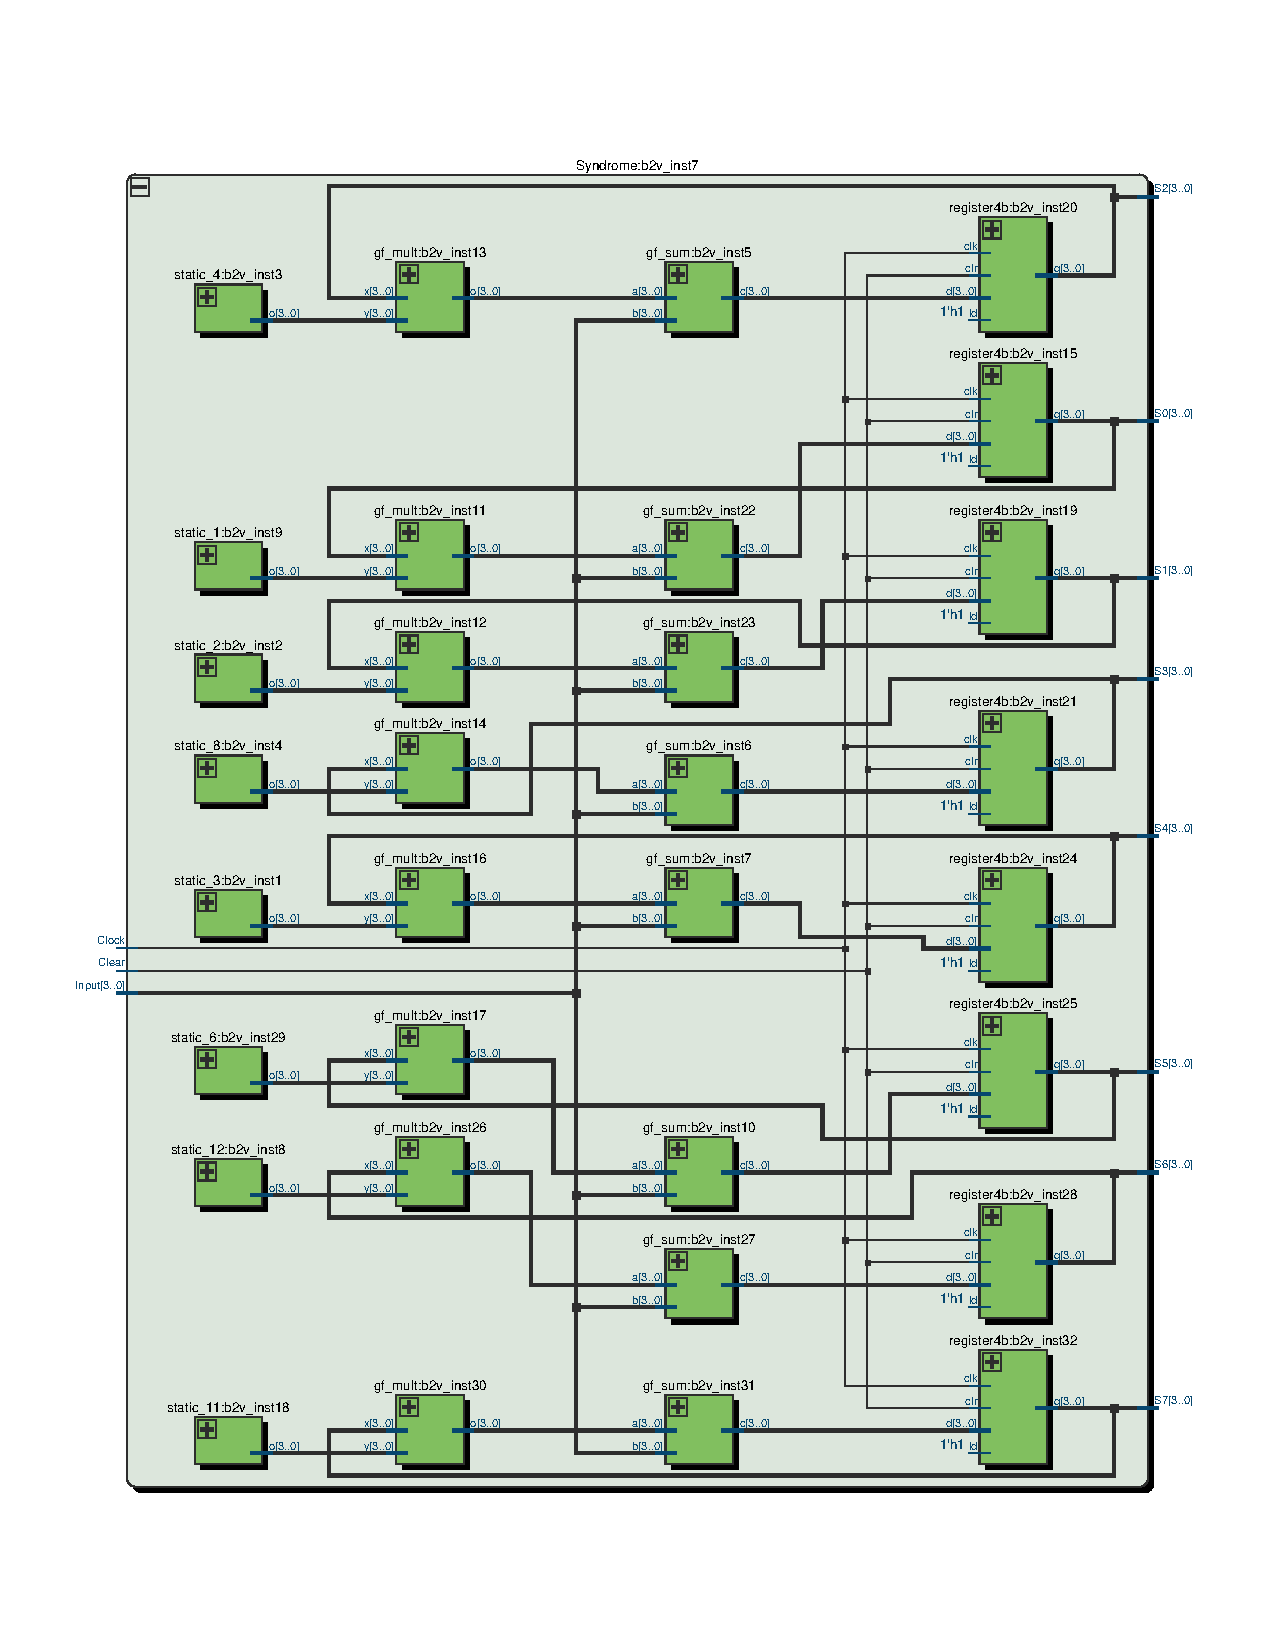
\includegraphics[width=0.5\textwidth, trim={0 1.2cm 0 3cm}, clip]{RS/SindromeRTL.pdf}
	\legend{Fonte: Autores.}
\end{figure}

\begin{figure}[h]
	\caption{\label{fig_berlekamp_arq}Arquitetura do módulo de Berlekamp-Massey.}
	\centering
	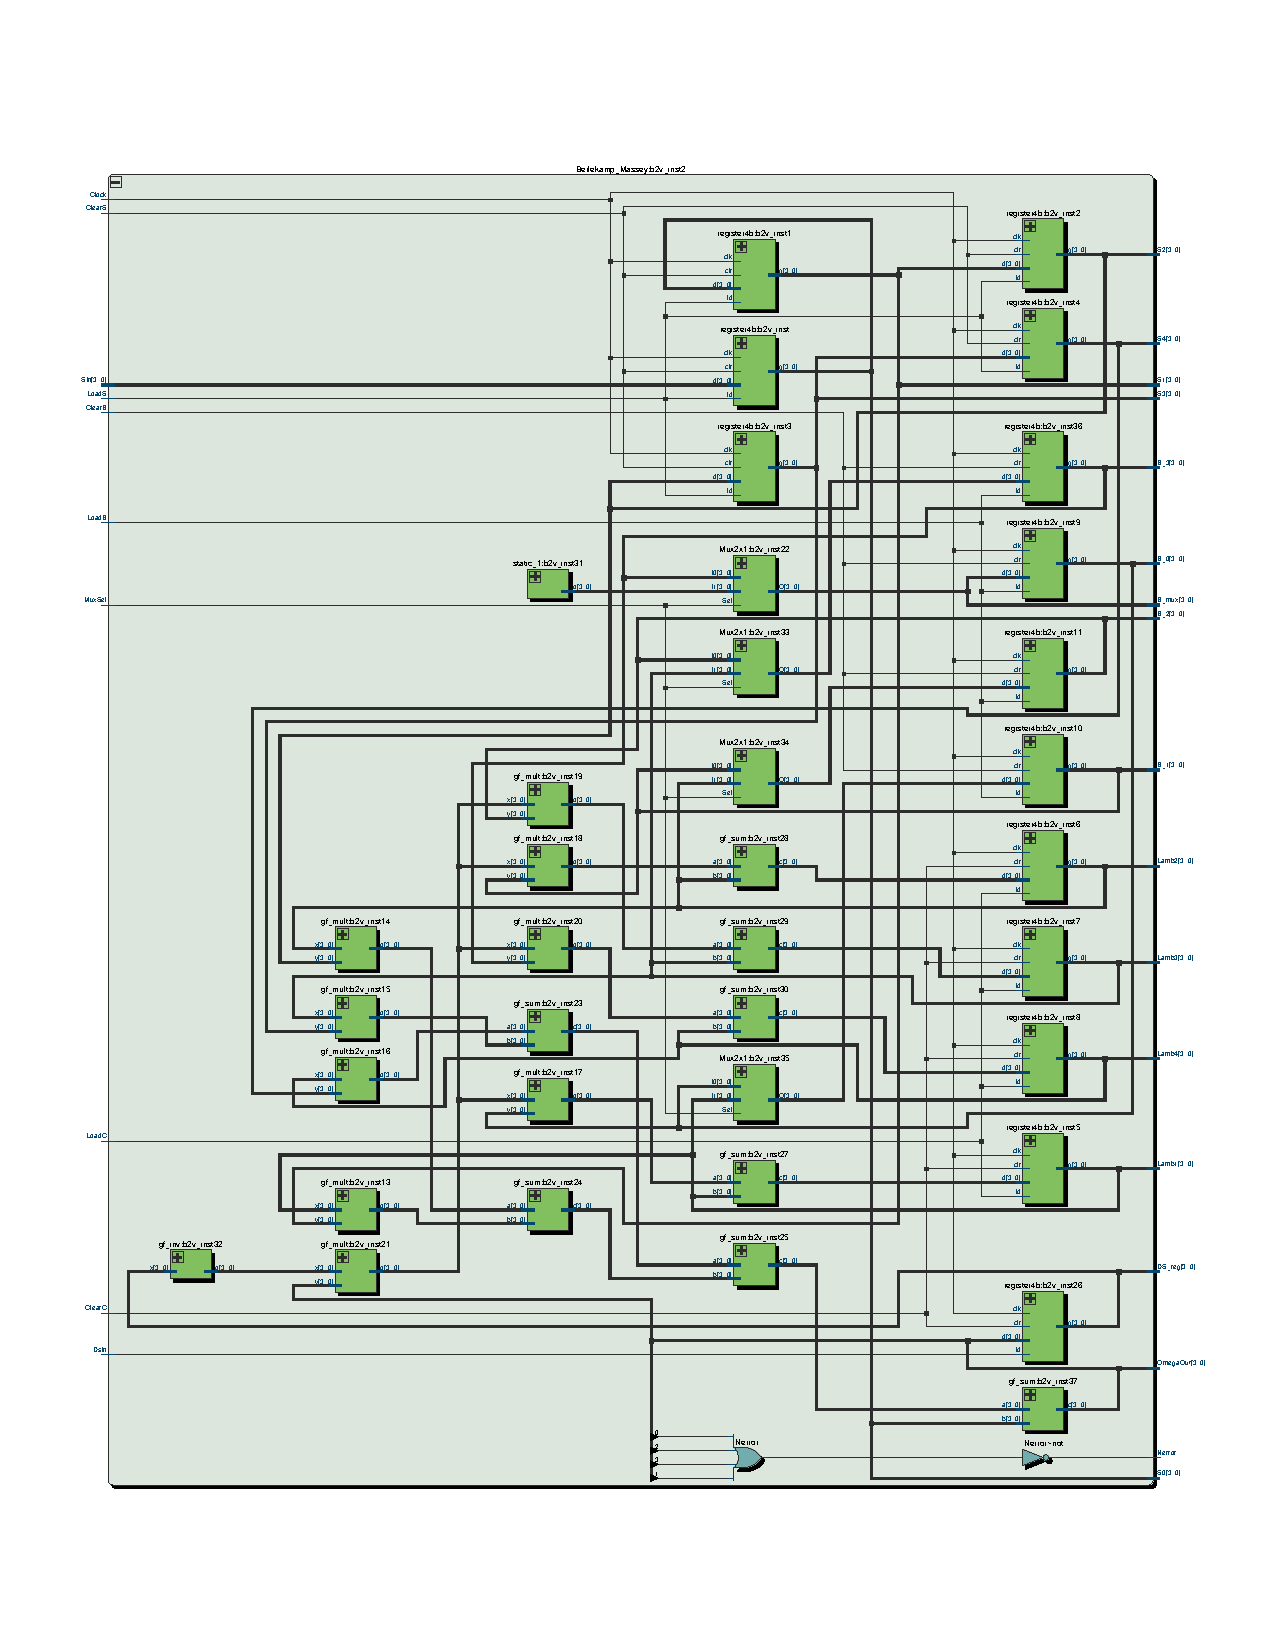
\includegraphics[width=0.5\textwidth, trim={0 1.2cm 0 3cm}, clip]{RS/BerlekampRTL.pdf}
	\legend{Fonte: Autores.}
\end{figure}

\begin{figure}[h]
	\caption{\label{fig_chienloc_arq}Arquitetura do módulo de busca de Chien: localização de erros.}
	\centering
	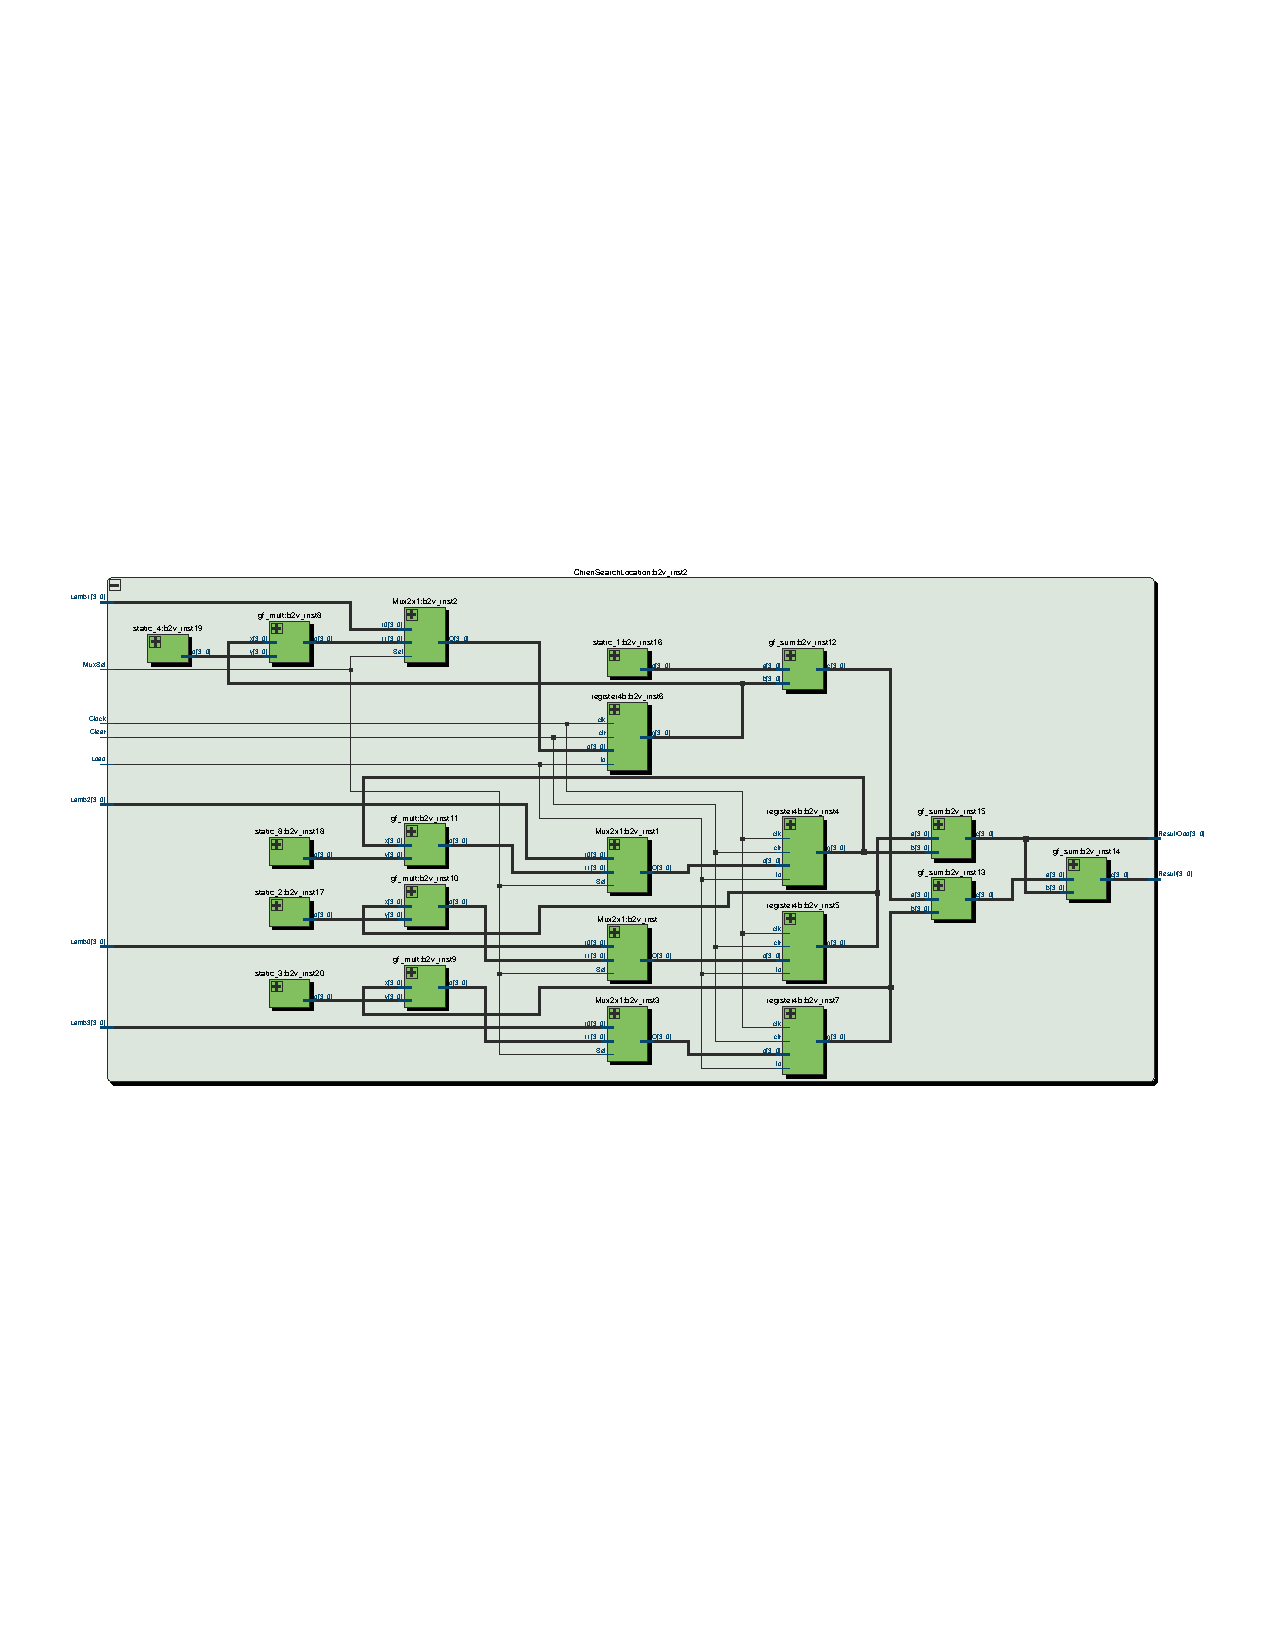
\includegraphics[width=0.5\textwidth, trim={0 8cm 0 9cm}, clip]{RS/ChienLocationRTL.pdf}
	\legend{Fonte: Autores.}
\end{figure}

\begin{figure}[h]
	\caption{\label{fig_chienval_arq}Arquitetura do módulo de busca de Chien: valores de erros.}
	\centering
	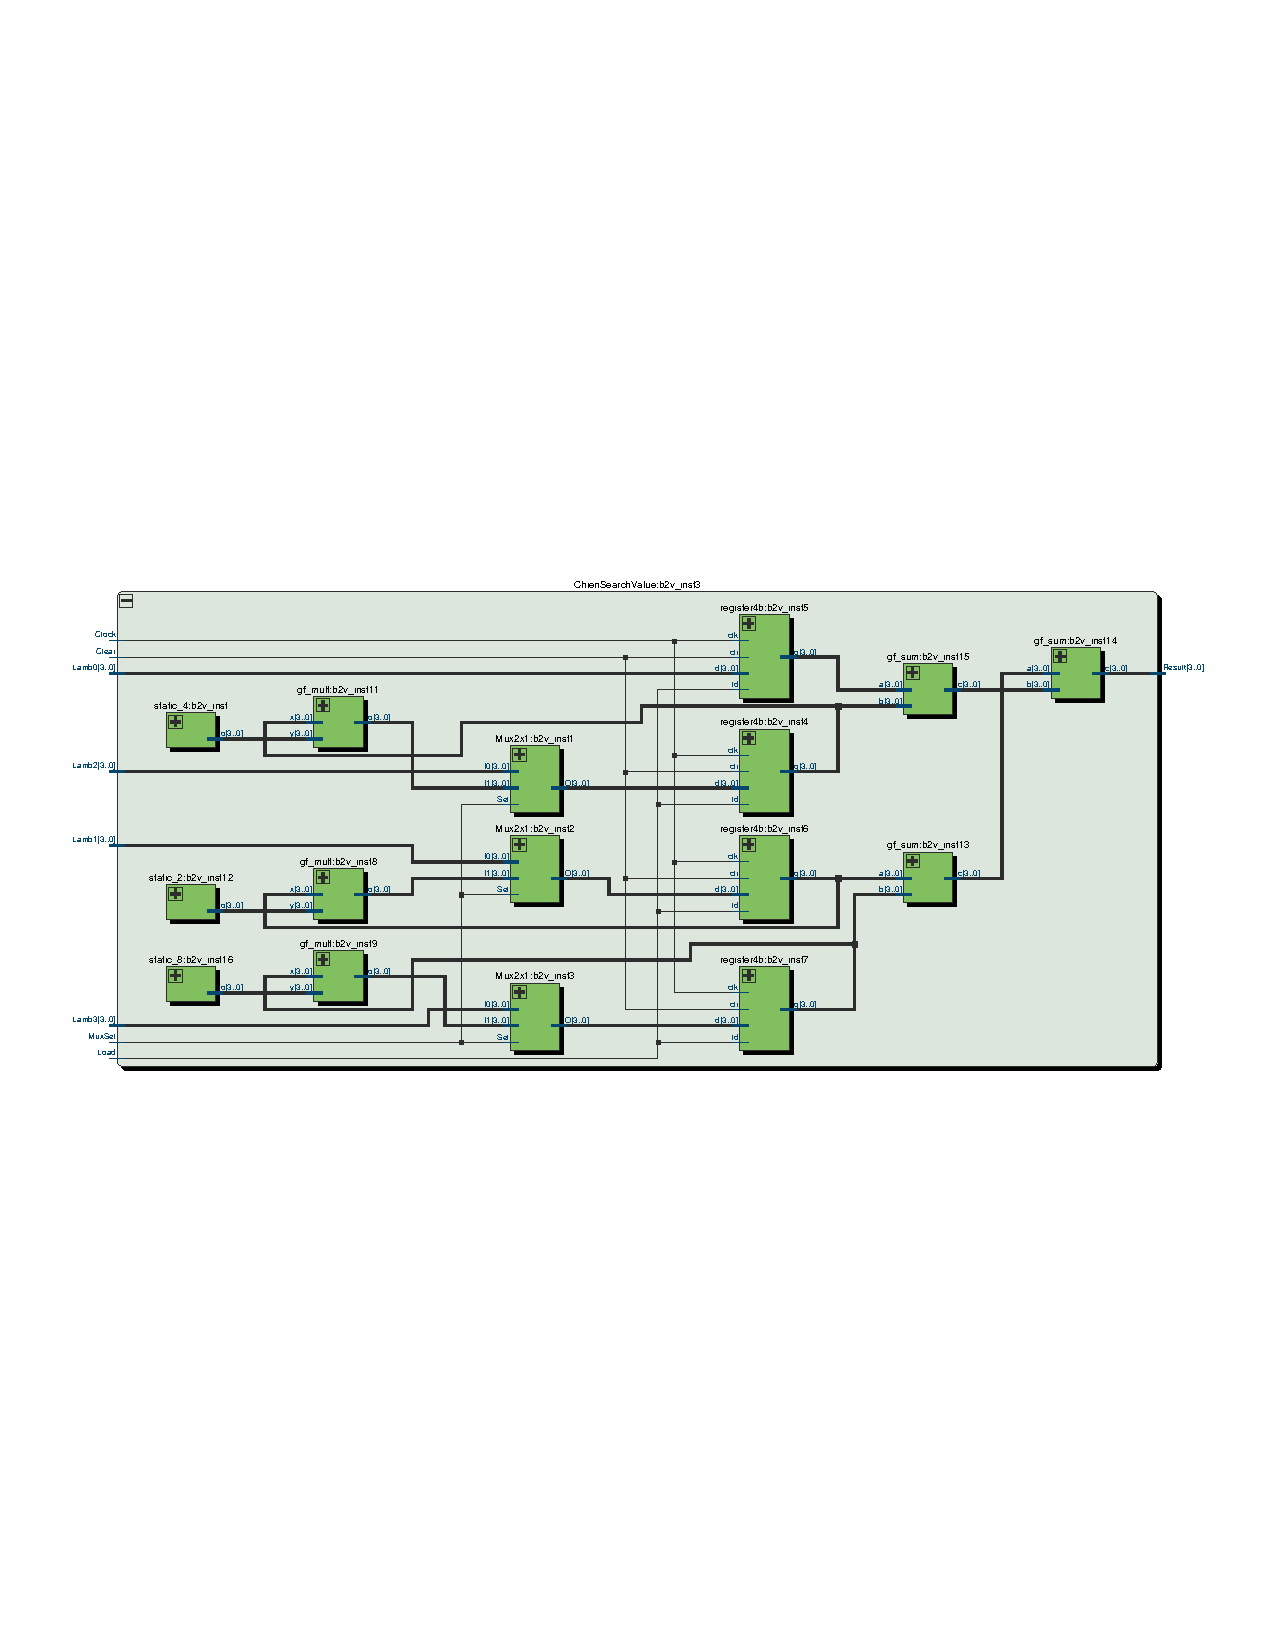
\includegraphics[width=0.5\textwidth, trim={0 8cm 0 9cm}, clip]{RS/ChienValueRTL.pdf}
	\legend{Fonte: Autores.}
\end{figure}

\begin{figure}[h]
	\caption{\label{figure:interleaver-rtl}Arquitetura do módulo de \textit{Interleaver}.}
	\centering
	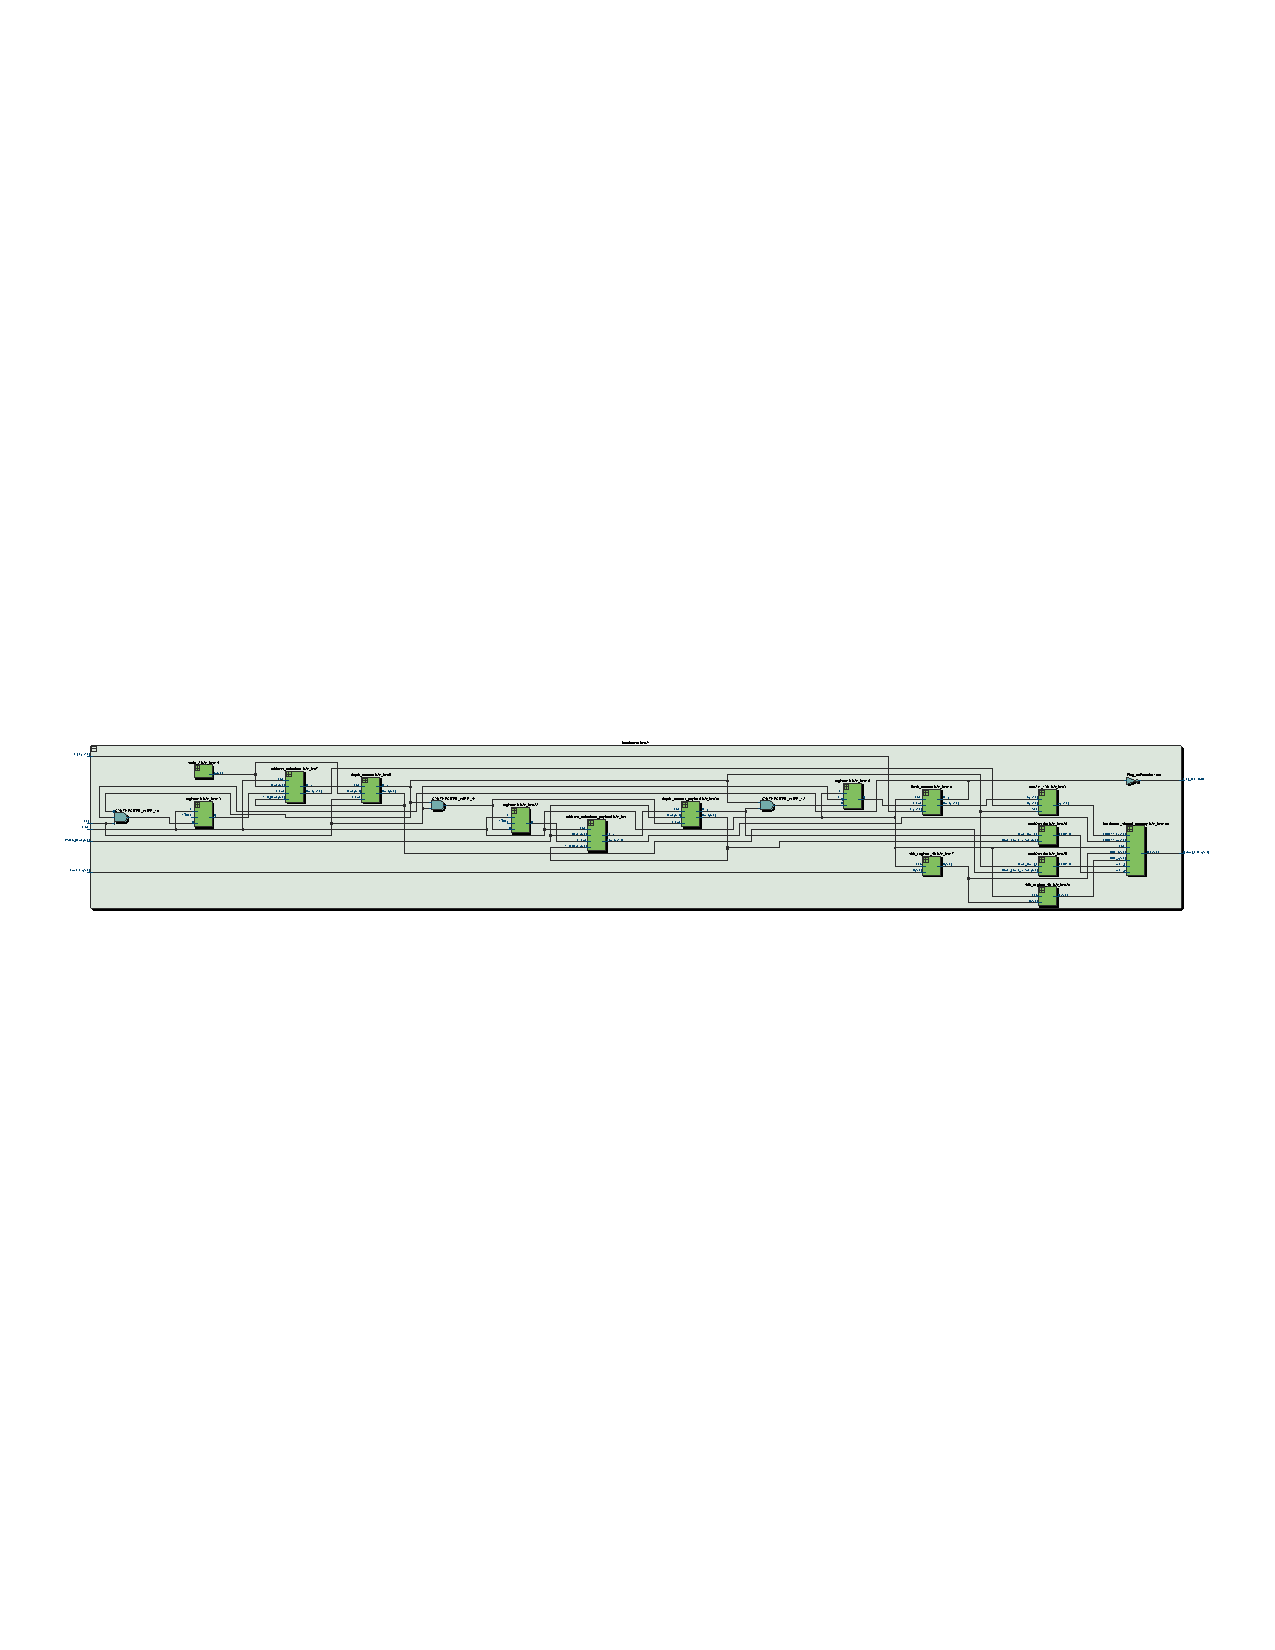
\includegraphics[width=1\textwidth, trim={0 12cm 0 12.5cm}, clip]{interleaver/rtl.pdf}
	\legend{Fonte: Autores.}
\end{figure}
\begin{figure}[h]
	\caption{\label{figure:sync-rtl}Arquitetura do módulo de Sincronização.}
	\centering
	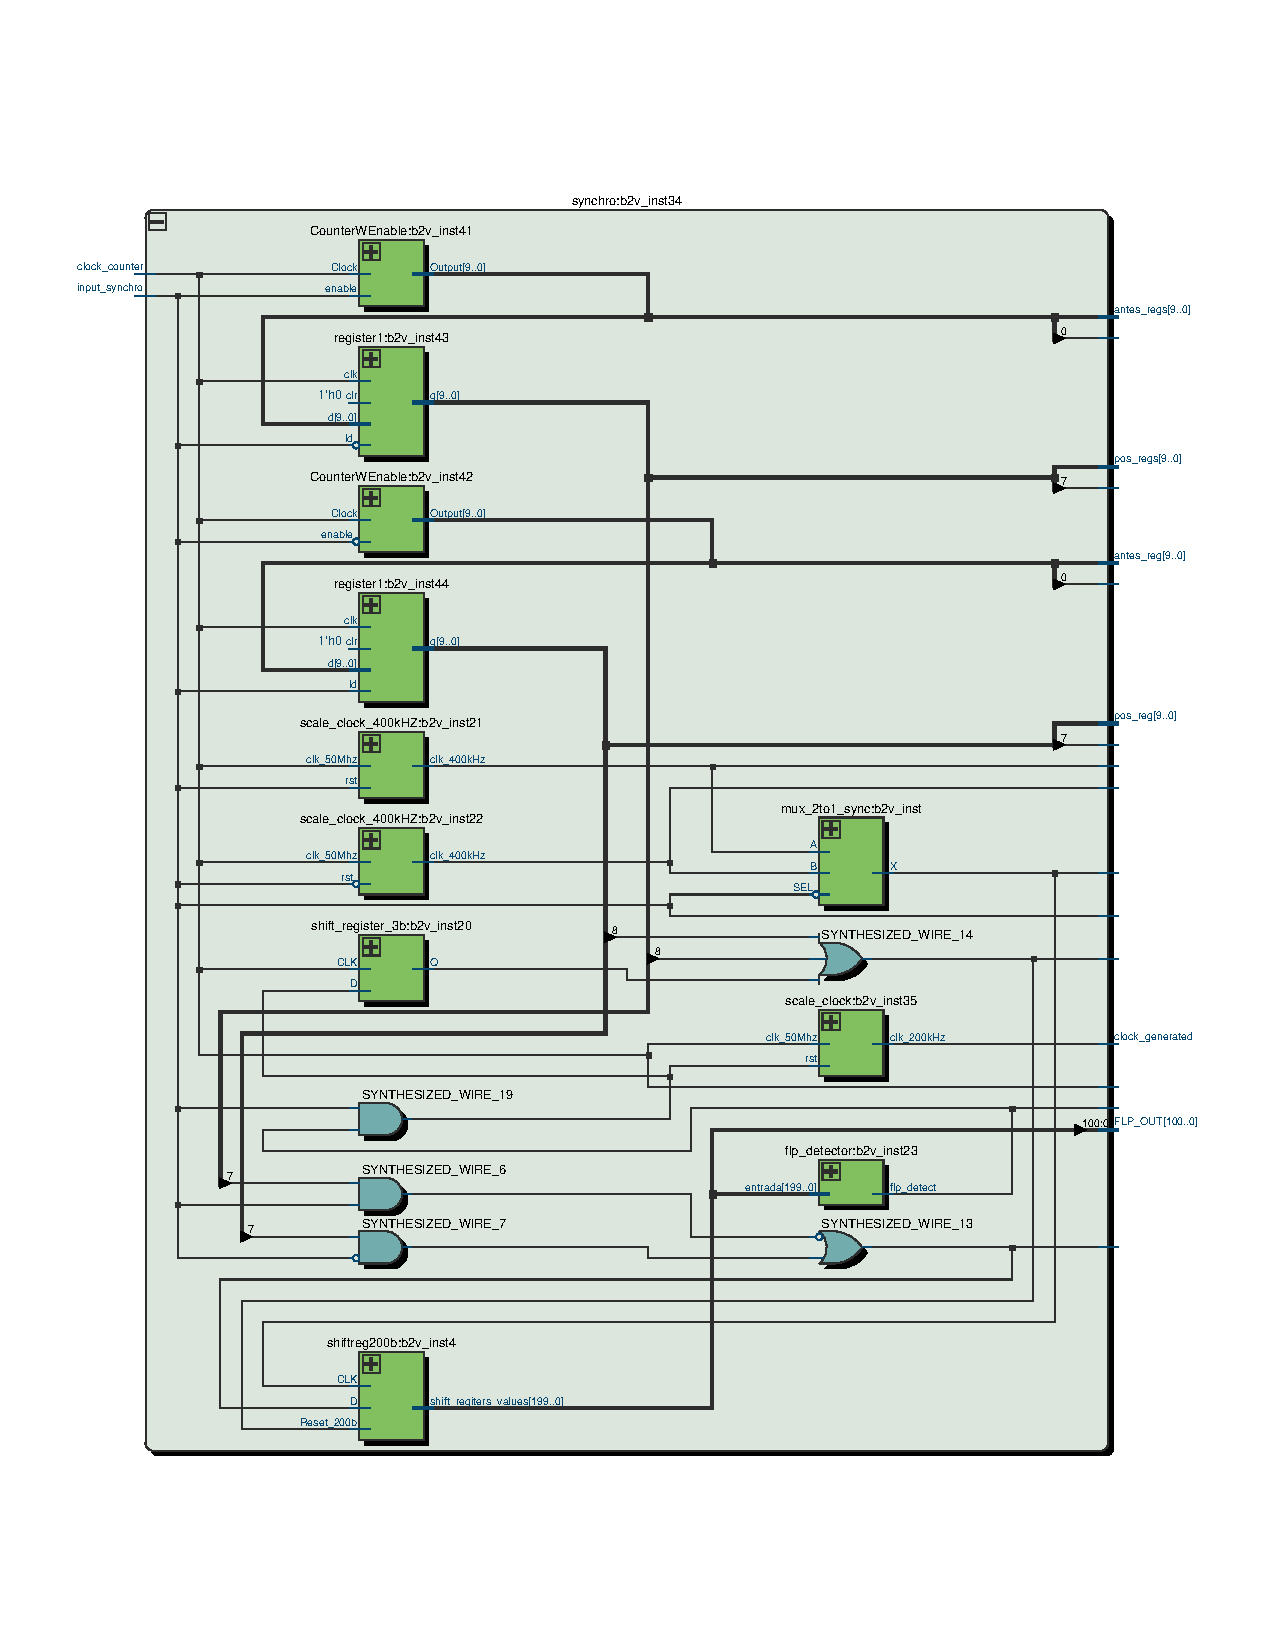
\includegraphics[width=0.5\textwidth, trim={0 2cm 0 3cm}, clip]{sync/rtl.pdf}
	\legend{Fonte: Autores.}
\end{figure}
\begin{figure}[h]
	\caption{\label{figure:manchester-decoder-rtl}Arquitetura do módulo de Decodificação Manchester.}
	\centering
	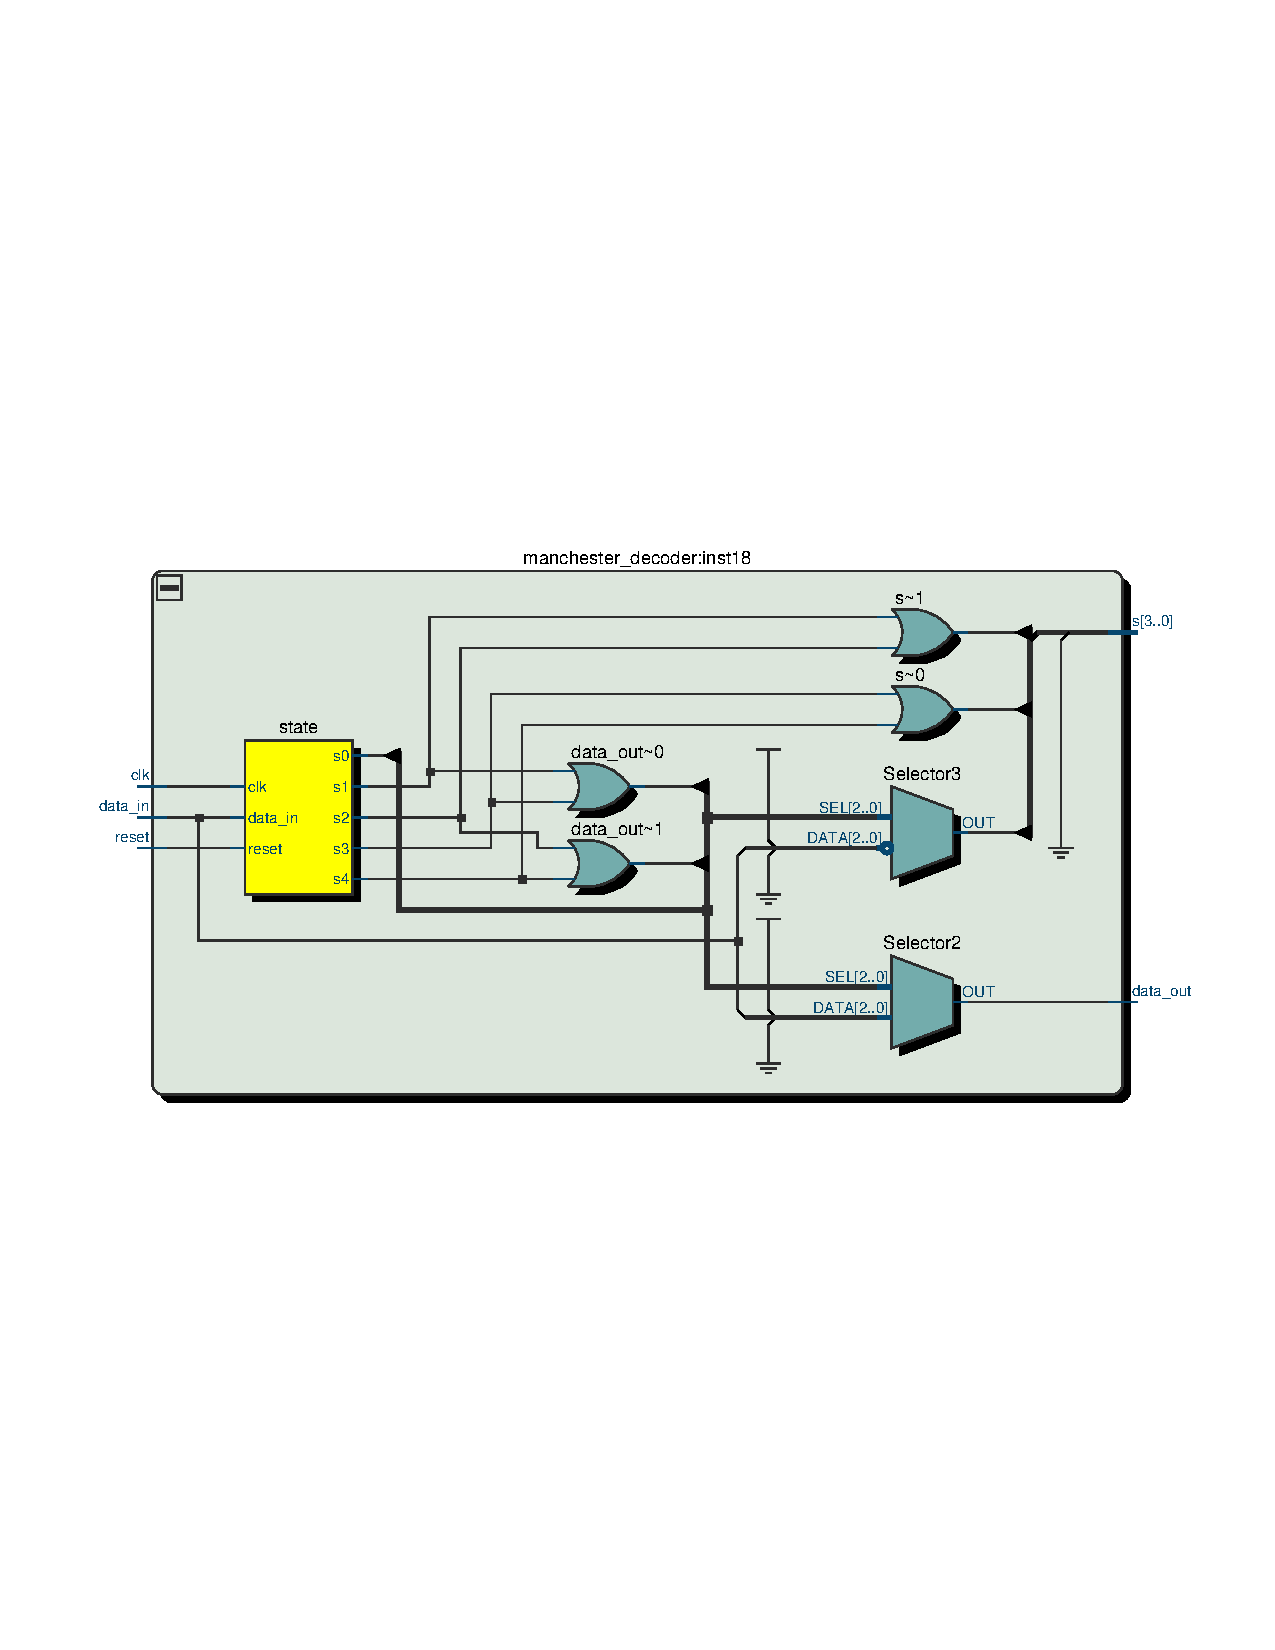
\includegraphics[width=0.5\textwidth, trim={0 7.7cm 0 8.5cm}, clip]{manchester/decoder-rtl.pdf}
	\legend{Fonte: Autores.}
\end{figure}

\begin{figure}[h]
	\caption{\label{figure:viterbi-rtl}Arquitetura do módulo de Decodificação Viterbi.}
	\centering
	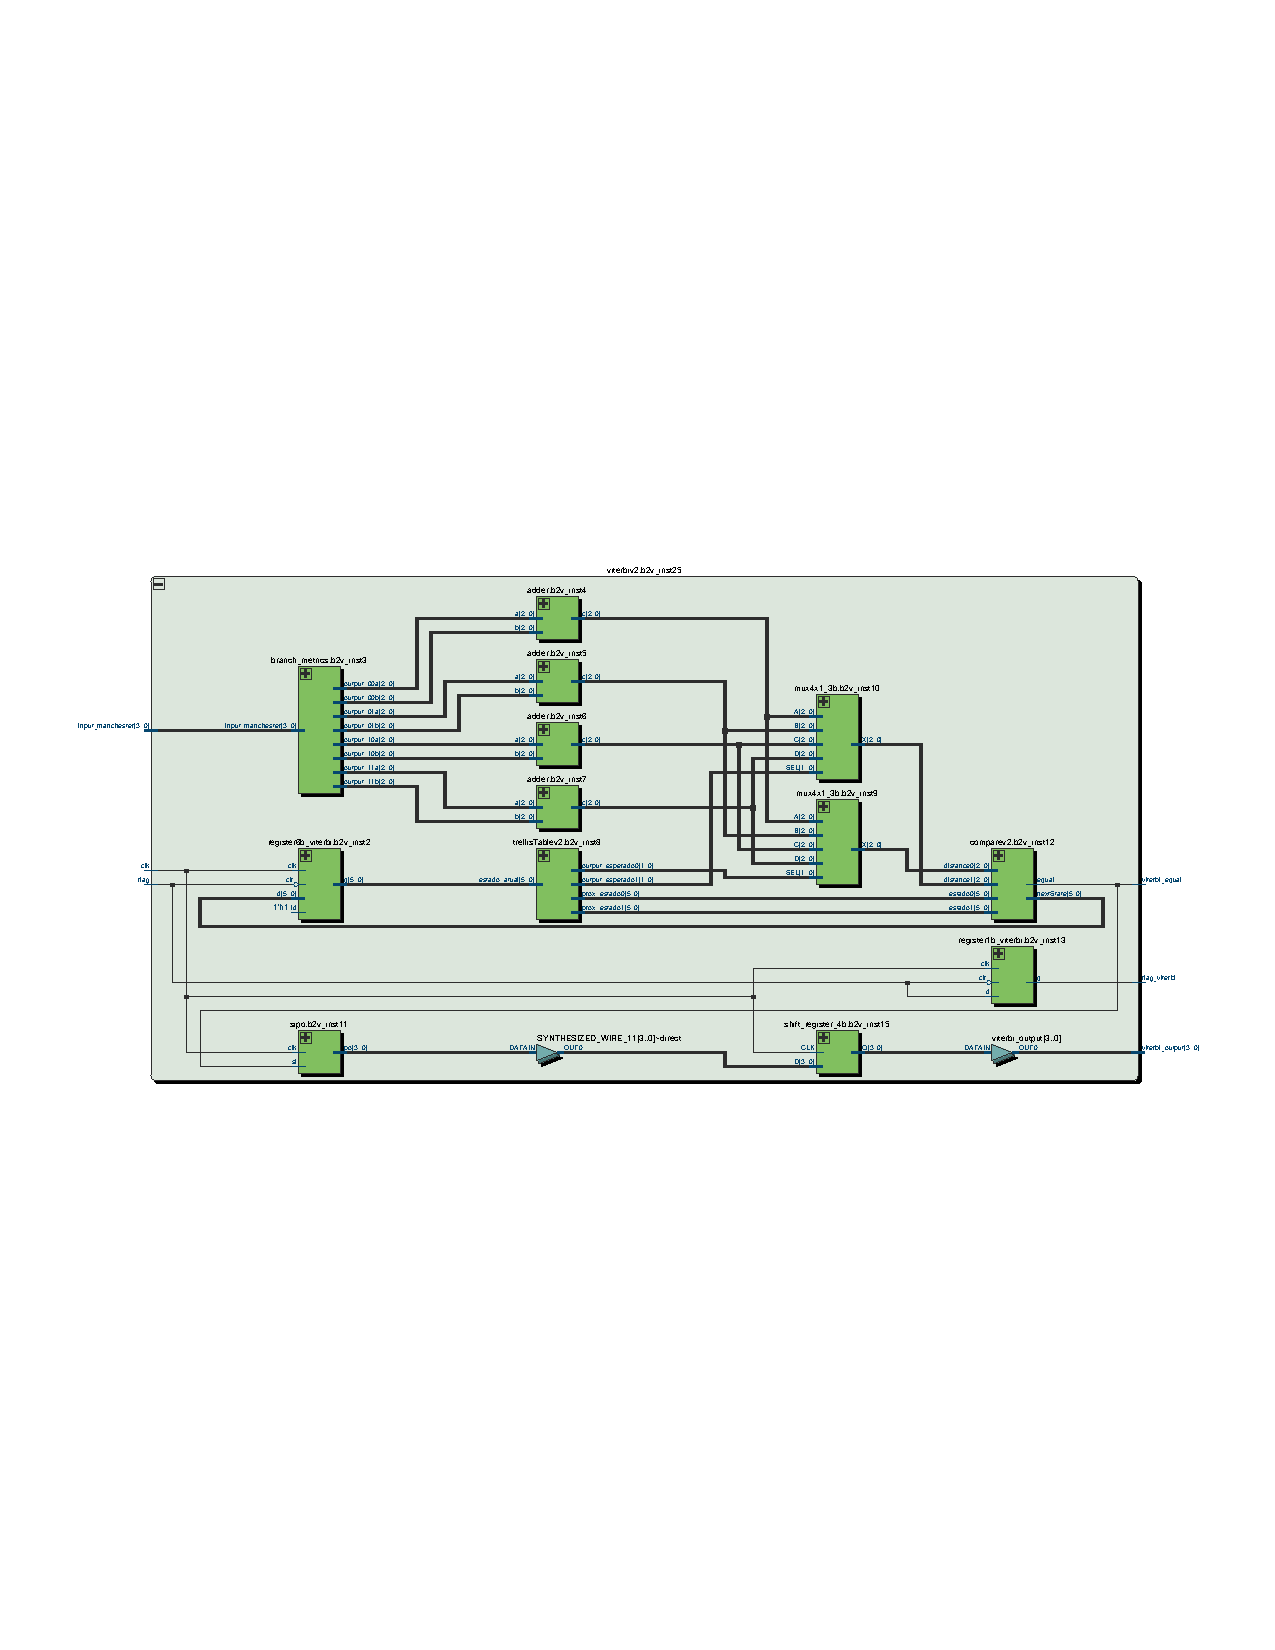
\includegraphics[width=0.5\textwidth, trim={0 7.7cm 0 8.5cm}, clip]{viterbi/rtl.pdf}
	\legend{Fonte: Autores.}
\end{figure}
	\end{apendicesenv}
	% ----------------------------------------------------------
	
	% ----------------------------------------------------------
	% Anexos - SEM ANEXOS
	% ----------------------------------------------------------
	%\begin{anexosenv}
		%\partanexos	% Imprime uma página indicando o início dos anexos
		%% ---
% Arquivo com os anexos do Trabalho de Conclusão de Curso dos alunos
% Gabriel Takaoka Nishimura, Felippe Demarqui Ramos e Vivian Kimie Isuyama 
% da Escola Politécnica da Universidade de São Paulo
% ---
\chapter{Diagramas da Arquitetura}

\begin{figure}[!htb]
	\caption{\label{fig_sindrome_arq}Arquitetura do módulo de cálculo das síndromes.}
	\centering%%trim={<left> <lower> <right> <upper>}
	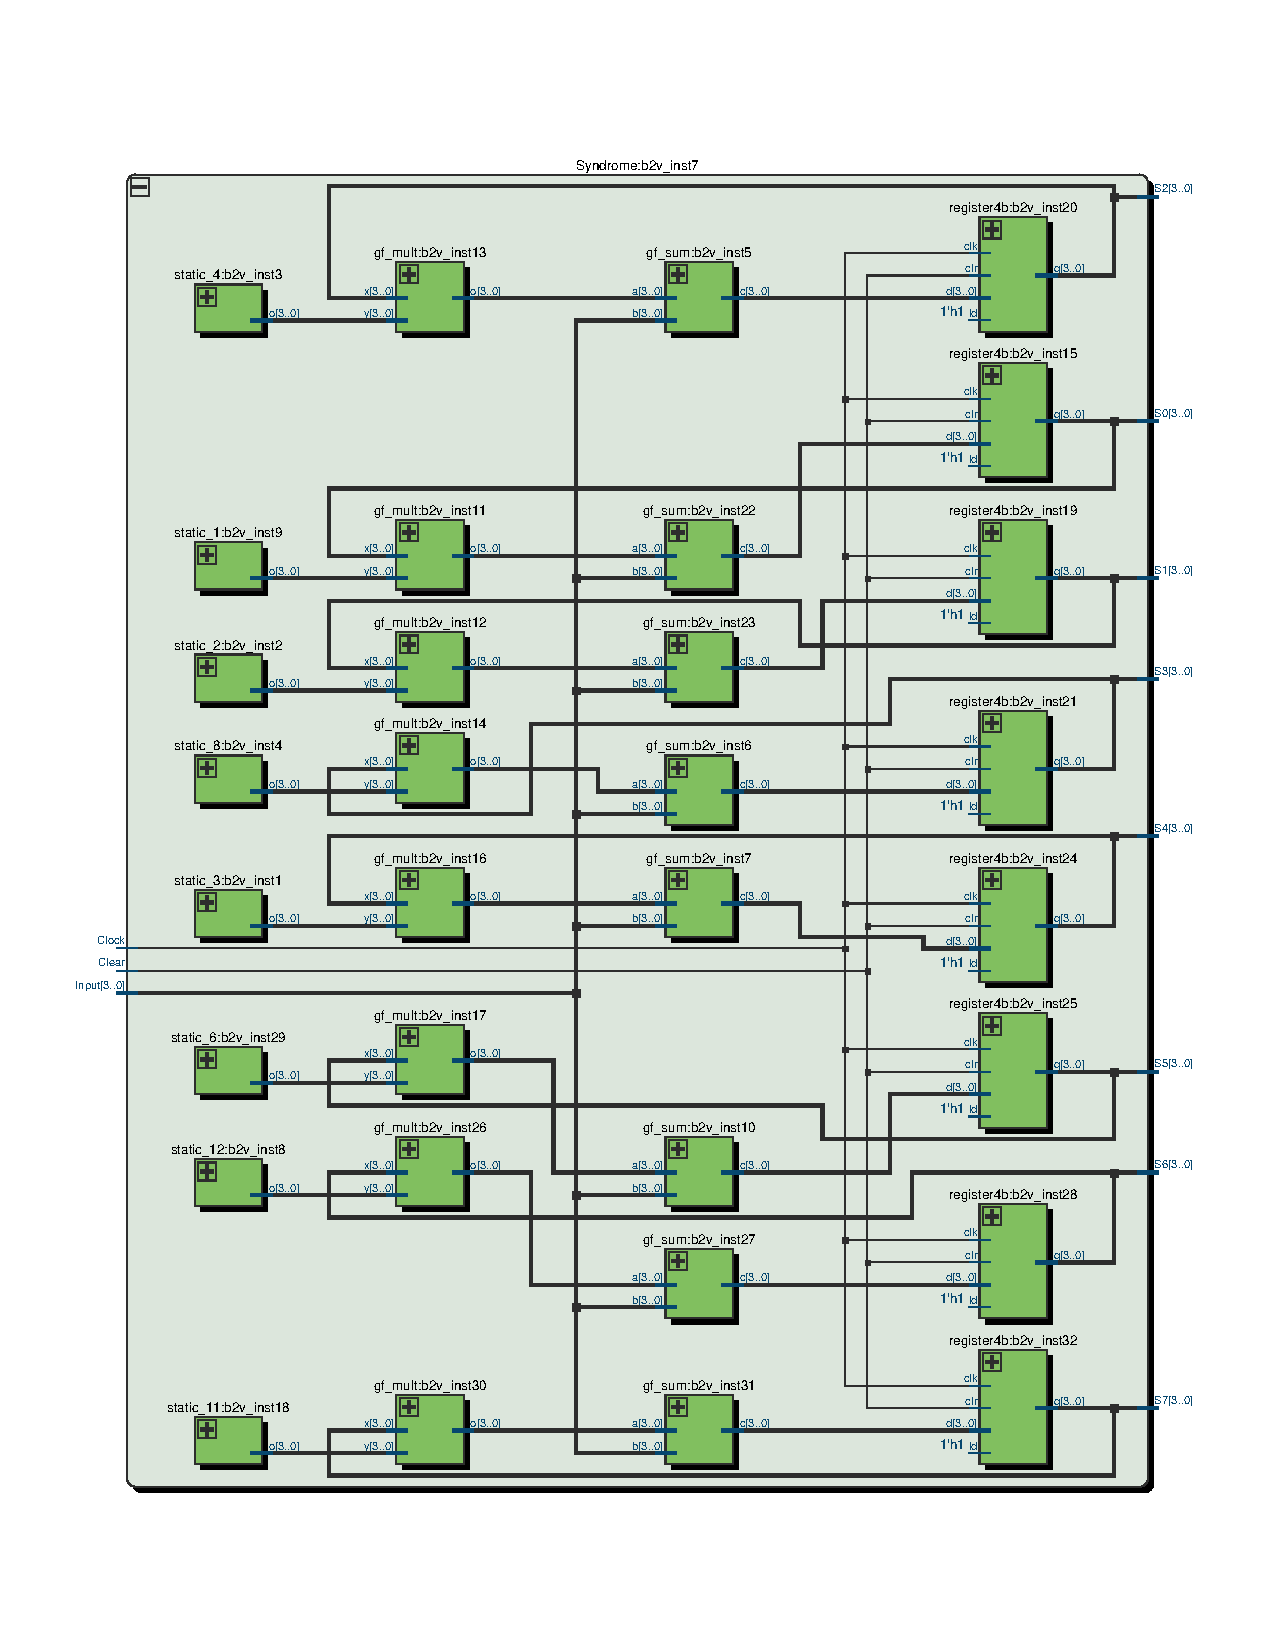
\includegraphics[width=1\textwidth, trim={2cm 5cm 2cm 5cm}]{RS/SindromeRTL.pdf}
	\legend{}
\end{figure}

\begin{figure}[!htb]
	\caption{\label{fig_berlekamp_arq}Arquitetura do módulo de Berlekamp-Massey.}
	\centering
	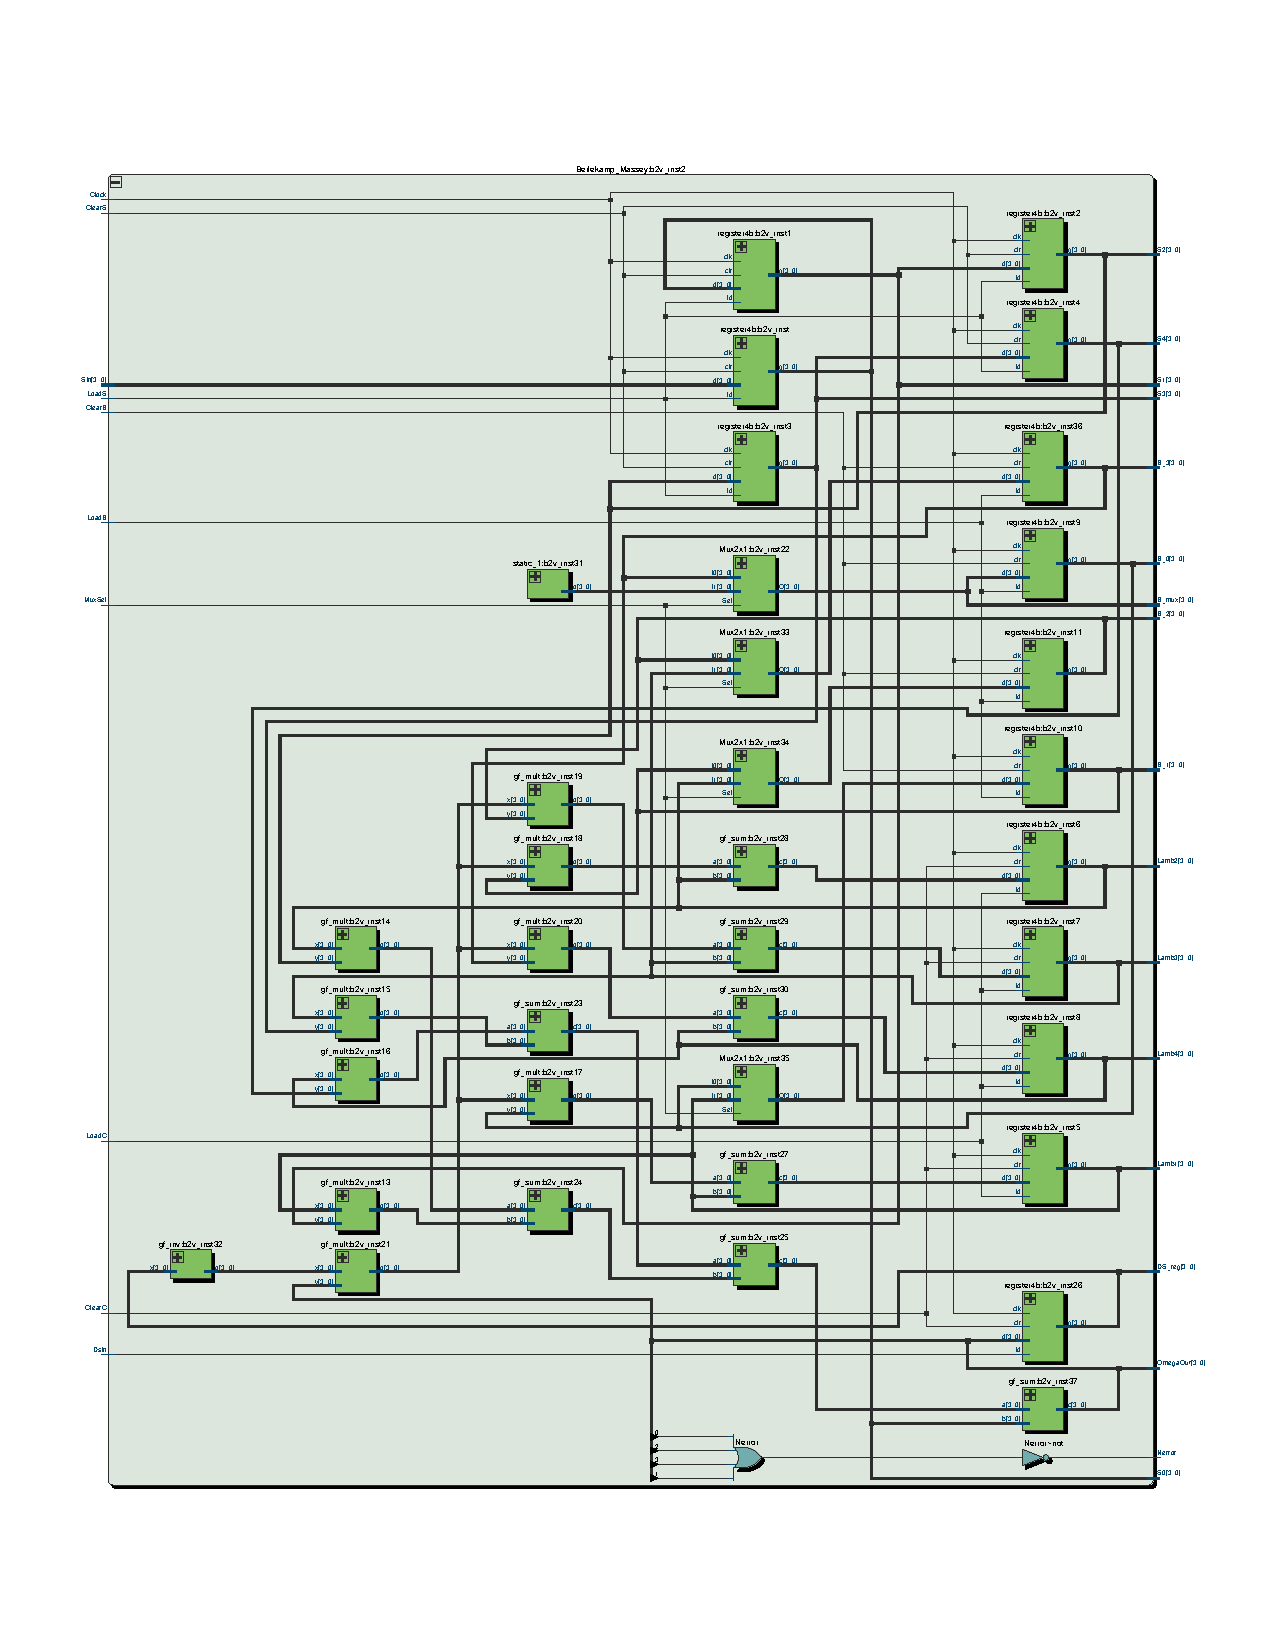
\includegraphics[width=1\textwidth, trim={2cm 5cm 2cm 5cm}]{RS/BerlekampRTL.pdf}
	\legend{}
\end{figure}

\begin{figure}[!htb]
	\caption{\label{fig_chienloc_arq}Arquitetura do módulo de busca de Chien: localização de erros.}
	\centering%%trim={<left> <lower> <right> <upper>}
	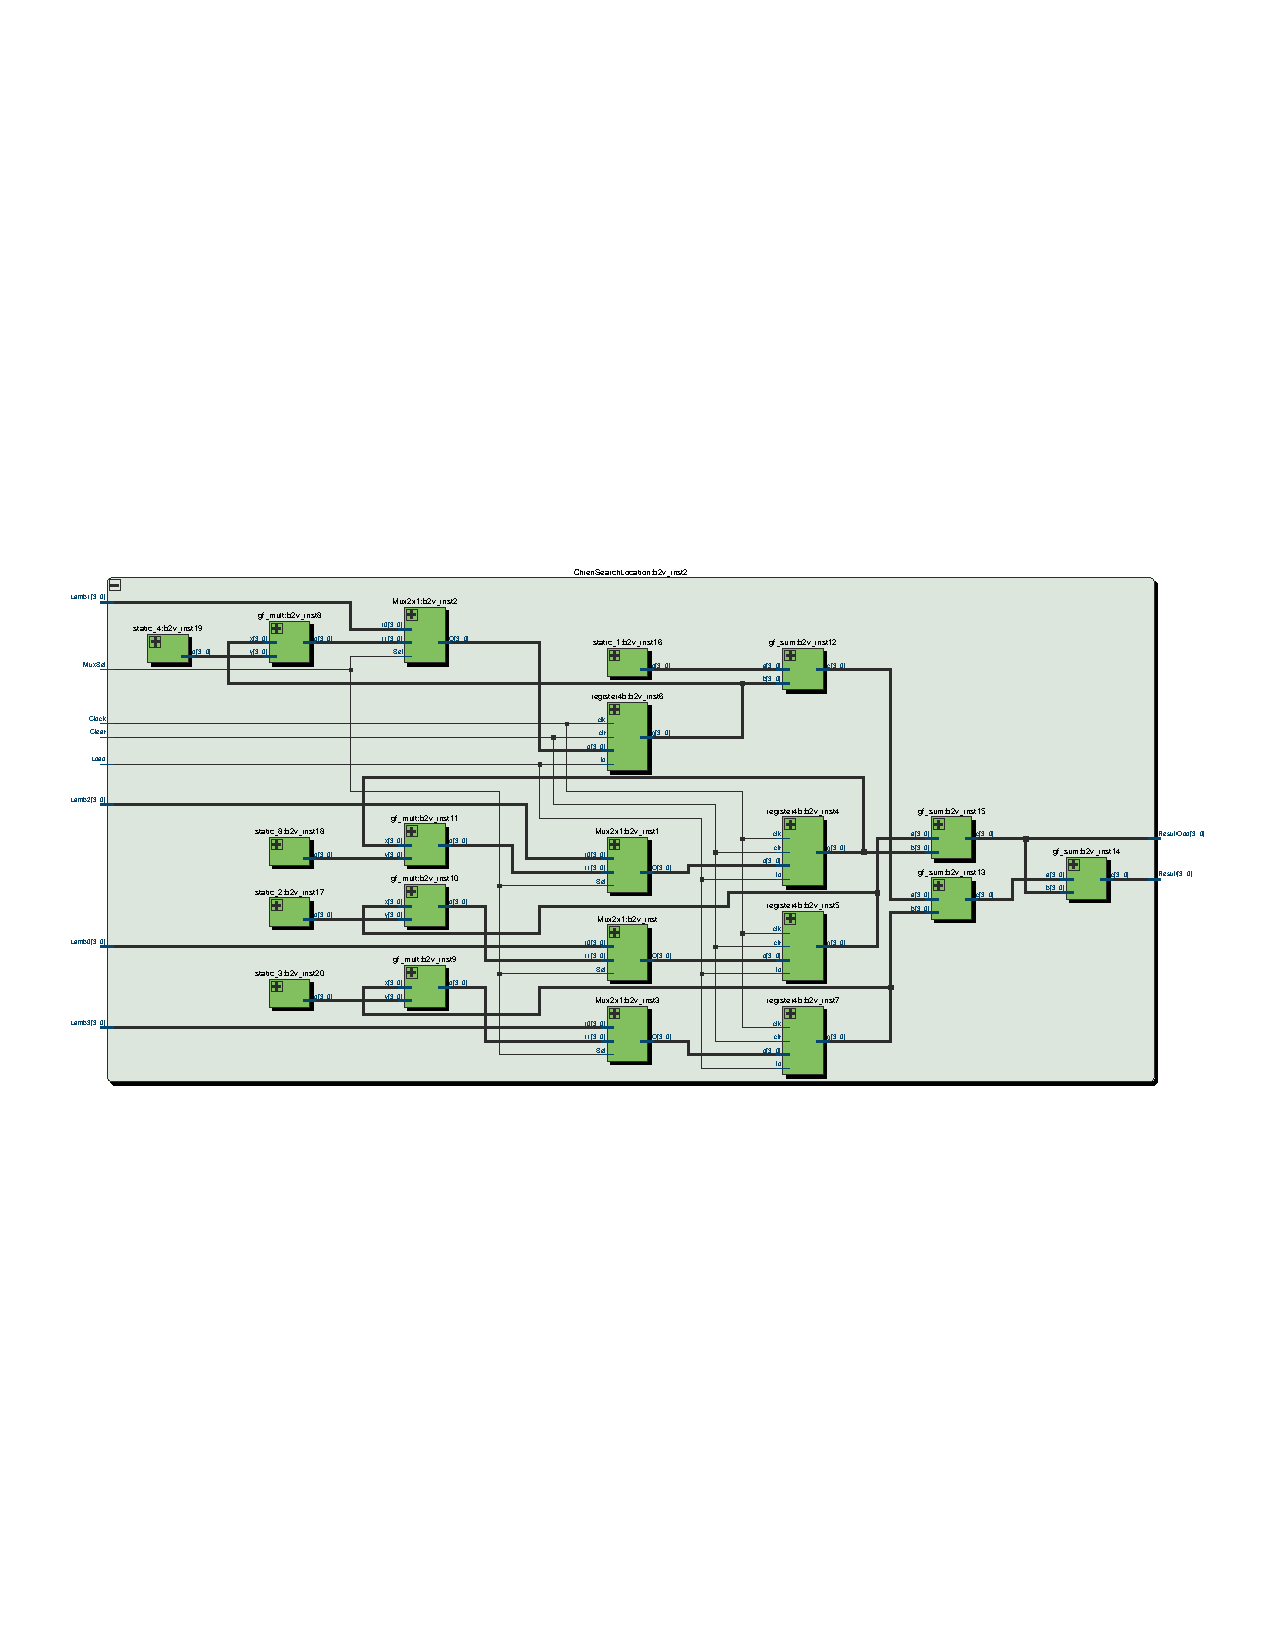
\includegraphics[width=1\textwidth, trim = {2cm 7cm 2cm 7cm}]{RS/ChienLocationRTL.pdf}
	\legend{}
\end{figure}

\begin{figure}[!htb]
	\caption{\label{fig_chienval_arq}Arquitetura do módulo de busca de Chien: valores de erros.}
	\centering %%trim={<left> <lower> <right> <upper>}
	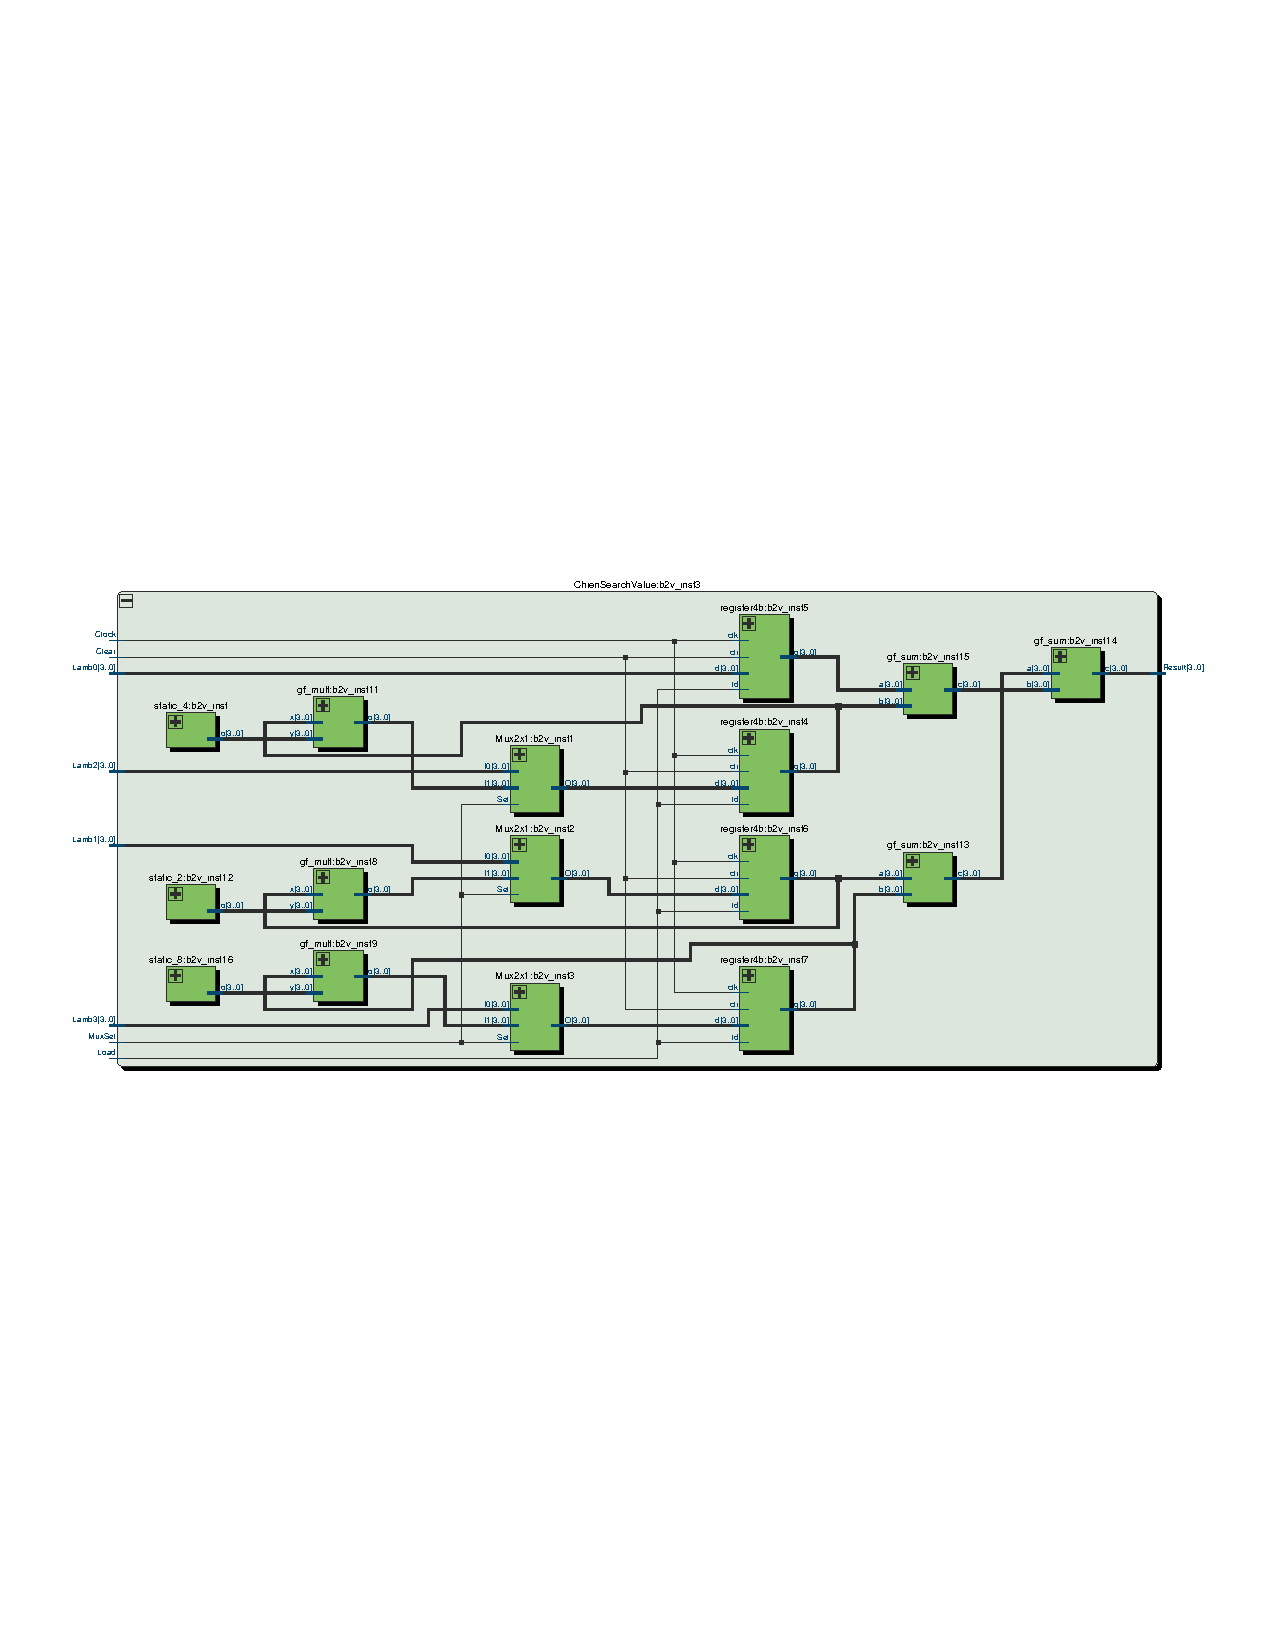
\includegraphics[width=1\textwidth,  trim = {2cm 7cm 2cm 7cm}]{RS/ChienValueRTL.pdf}
	\legend{}
\end{figure}
	%\end{anexosenv}
	% ----------------------------------------------------------
	
	%---------------------------------------------------------------------
	% INDICE REMISSIVO
	%---------------------------------------------------------------------
	\phantompart
	\printindex
	%---------------------------------------------------------------------
	
\end{document}